\chapter{Лекция 2. Отношения эквивалентности. Отношения порядка}

% === Отношения эквивалентности ===

\begin{defn}{Отношение эквивалентности}{equiv-rel}
$M \neq \varnothing$,\; $f\colon M^2 \to \mathbb{B}$.

$f$ --- \textbf{отношение эквивалентности} $\;\Leftrightarrow\;$
$f$ рефлексивно, симметрично и транзитивно.
\end{defn}

\textbf{Пример.} Список присутствующих:
$f(a,b) = 1 \;\Leftrightarrow\;$ первая буква фамилии $a$ совпадает
с первой буквой фамилии $b$.

Все фамилии разбиваются на классы: $\text{А}, \text{Б}, \ldots$

\textbf{Пример.} $M = \mathbb{Z}$, операция сравнения по модулю $n$:
$f(a,b) = 1 \;\Leftrightarrow\; a \equiv b \pmod{n}$.

Классы эквивалентности:
\[
  \mathcal{E} = \mathcal{E}_0 \cup \mathcal{E}_1 \cup \ldots \cup \mathcal{E}_{n-1}.
\]

\begin{defn}{Класс эквивалентности}{equiv-class}
$M \neq \varnothing$,\; $f$ --- эквивалентность на $M$.

$\forall\, a \in M$ \textbf{класс эквивалентности} элемента $a$:
\[
  H_a := \bigl\{\, c \in M \;\big|\; f(a, c) = 1 \,\bigr\}.
\]
\end{defn}

\begin{statement}{Теорема о классификации}{classification-thm}
$M \neq \varnothing$,\; $f$ --- эквивалентность на $M$. Тогда:
\begin{enumerate}
  \item $\forall\, a \in M\colon\; a \in H_a$.
  \item $\forall\, a, b \in M\colon\;
        H_a \cap H_b = \varnothing \;\text{ или }\; H_a = H_b$.
  \item $M = \bigcup\limits_{i} H_{a_i}$.
\end{enumerate}
\end{statement}

\begin{proof}
Напомним, что класс элемента $a$ --- это $H_a=\{x\in M\colon f(a,x)=1\}$.

\textbf{1) Каждый элемент лежит в своём классе.} В силу рефлексивности
$f(a,a)=1$, поэтому $a\in H_a$; в частности, $H_a\neq\varnothing$.

\textbf{2) Два класса либо не пересекаются, либо совпадают.} Пусть
$H_a\cap H_b\neq\varnothing$; покажем, что тогда $H_a=H_b$. Возьмём
$c\in H_a\cap H_b$, то есть $f(a,c)=1$ и $f(b,c)=1$. Докажем включение
$H_a\subseteq H_b$. Пусть $x\in H_a$, т.\,е. $f(a,x)=1$. По симметричности из
$f(a,c)=1$ получаем $f(c,a)=1$; тогда по транзитивности
$f(c,a)=1\wedge f(a,x)=1\Rightarrow f(c,x)=1$. Наконец, $f(b,c)=1$ и
$f(c,x)=1$ дают по транзитивности $f(b,x)=1$, то есть $x\in H_b$. Значит
$H_a\subseteq H_b$; симметрично $H_b\subseteq H_a$, поэтому $H_a=H_b$. Итак,
два класса либо совпадают, либо не пересекаются.

\textbf{3) Классы покрывают всё множество.} По пункту~1 каждый элемент
$a\in M$ лежит в своём классе $H_a$, поэтому
$M\subseteq\bigcup_{a\in M}H_a\subseteq M$, откуда $M=\bigcup_{a\in M}H_a$.
Выбрав по одному представителю из каждого попарно различного класса
(по пункту~2 различные классы не пересекаются), получаем разбиение
$M=\bigsqcup_i H_{a_i}$ на непустые непересекающиеся классы. Это и есть
искомая классификация.
\end{proof}

\medskip
\textbf{Граф и матрица отношения эквивалентности.}

Граф отношения эквивалентности распадается на полные подграфы
(клики) --- классы эквивалентности.

\textit{Пример.} Вершины $m_1, m_2$ образуют один класс (полный подграф с петлями),
вершины $n_1, n_2, n_3, n_4$ --- другой класс (полный подграф с петлями).

Матрица смежности (в порядке $m_1, m_2, n_1, n_2, n_3, n_4$) имеет
блочно-диагональный вид:
\begin{center}
\renewcommand{\arraystretch}{1.25}
$A_f=$\;
\begin{tabular}{|c||c|c||c|c|c|c|}
\hline
$f$ & $m_1$ & $m_2$ & $n_1$ & $n_2$ & $n_3$ & $n_4$ \\ \hline\hline
$m_1$ & 1 & 1 & 0 & 0 & 0 & 0 \\ \hline
$m_2$ & 1 & 1 & 0 & 0 & 0 & 0 \\ \hline\hline
$n_1$ & 0 & 0 & 1 & 1 & 1 & 1 \\ \hline
$n_2$ & 0 & 0 & 1 & 1 & 1 & 1 \\ \hline
$n_3$ & 0 & 0 & 1 & 1 & 1 & 1 \\ \hline
$n_4$ & 0 & 0 & 1 & 1 & 1 & 1 \\ \hline
\end{tabular}
\end{center}
\noindent Двойные линии выделяют блоки: матрица имеет блочно-диагональный
вид, каждый блок --- отдельный класс эквивалентности (вне блоков --- нули).

\bigskip
% === Отношения порядка ===
\subsection*{Отношения порядка}

\begin{defn}{Частичный (нестрогий) порядок}{partial-order}
$M \neq \varnothing$,\; $f\colon M^2 \to \mathbb{B}$.

$f$ --- \textbf{частичный (нестрогий) порядок}
$\;\Leftrightarrow\;$ $f$ рефлексивно, антисимметрично и транзитивно.
\end{defn}

\textbf{Примеры частичного порядка.}

\begin{enumerate}
  \item $\mathbb{R}$, $\leq$ --- обычный порядок на вещественных числах.

  \item $M = \mathbb{B}^3$ (3-мерные двоичные векторы).

        $\alpha = a_1 a_2 a_3$,\; $\beta = b_1 b_2 b_3$.
        \[
          \alpha \leq \beta \;\Leftrightarrow\;
          a_i \leq b_i,\quad 1 \leq i \leq 3.
        \]

  \item $N = \{a, b\}$,\; $M$ --- все возможные подмножества $N$
        (т.\,е. $M = 2^N = \{\varnothing, \{a\}, \{b\}, \{a,b\}\}$).

        $f\colon M^2 \to \mathbb{B}$,\quad
        $\forall\, A, B \in M\colon\; f(A,B) = 1 \;\Leftrightarrow\; A \subseteq B$.
\end{enumerate}

\medskip
Отношение эквивалентности --- для \textit{классификации},
отношение порядка --- для \textit{иерархии}.

\medskip
\textbf{Граф} (пример~3). $M = \{\varnothing,\, \{a\},\, \{b\},\, \{a,b\}\}$ ---
диаграмма Хассе. Независимые элементы ($\{a\}$ и $\{b\}$) ---
условия непонятно как соотносятся между собой.

Матрица смежности (в порядке $\varnothing, \{a\}, \{b\}, \{a,b\}$):
\begin{center}
\renewcommand{\arraystretch}{1.25}
$A_f=$\;
\begin{tabular}{|c||*{4}{c|}}
\hline
$f(a,b)$ & $\varnothing$ & $\{a\}$ & $\{b\}$ & $\{a,b\}$ \\ \hline\hline
$\varnothing$  & 1 & 1 & 1 & 1 \\ \hline
$\{a\}$        & 0 & 1 & 0 & 1 \\ \hline
$\{b\}$        & 0 & 0 & 1 & 1 \\ \hline
$\{a,b\}$      & 0 & 0 & 0 & 1 \\ \hline
\end{tabular}
\end{center}

\begin{defn}{Линейный порядок}{linear-order}
$M \neq \varnothing$,\; $f\colon M^2 \to \mathbb{B}$.

$f$ --- \textbf{линейный порядок} $\;\Leftrightarrow\;$
$f$ --- частичный порядок и
$\forall\, a, b \in M\colon\; f(a,b) = 1 \;\vee\; f(b,a) = 1$.
\end{defn}

\medskip
\textbf{Алгоритм дополнения частичного порядка до линейного.}

\textit{Дано:} $M \neq \varnothing$,\; $f\colon M^2 \to \mathbb{B}$,\; $f$ --- ч.\,п.

\textit{Построить:} $\tilde{f}$ --- линейный порядок на $M$, согласованный с $f$:
\[
  \forall\, a, b \in M\colon\;
  f(a,b) = 1 \;\Rightarrow\; \tilde{f}(a,b) = 1.
\]
Способ не один!

\bigskip
\textbf{DFS} (поиск в глубину) --- обход дерева/графа с использованием стека (FILO).

% Граф: dfs-example.graph (12 вершин, нумерация по порядку DFS-обхода)
\grfig{figures/dfs-example.pdf}{Граф 12 вершин, нумерация DFS-обхода}

\textbf{BFS} (поиск в ширину) --- обход дерева/графа по уровням
с использованием очереди (FIFO).

% Граф: bfs-example.graph (тот же граф, нумерация по порядку BFS-обхода)
\grfig{figures/bfs-example.pdf}{Тот же граф, нумерация BFS-обхода}

% Обходы графа: DFS и BFS (визуализация шагов)
% ============================================================
\needspace{14\baselineskip}\subsection*{Обходы графа: поиск в глубину и в ширину}

\begin{algo}{Поиск в глубину (DFS) и поиск в ширину (BFS)}{dfs-bfs}
\textbf{Поиск в глубину (DFS)} использует стек: из текущей вершины уходим как
можно глубже, и только упёршись в тупик, возвращаемся назад. \textbf{Поиск в
ширину (BFS)} использует очередь: сначала обрабатываются все соседи текущей
вершины, затем соседи соседей — обход идёт «слоями».

\medskip
\noindent\textbf{Цветовые обозначения на рисунках:} текущая (активная) вершина
— оранжевая, уже в стеке/очереди — синяя, обработанная — зелёная; рёбра дерева
обхода выделены зелёным.

\medskip
\noindent\textbf{Пример работы DFS} (старт из $S$):

\begin{center}\begin{tabular}{ccc}
\shortstack{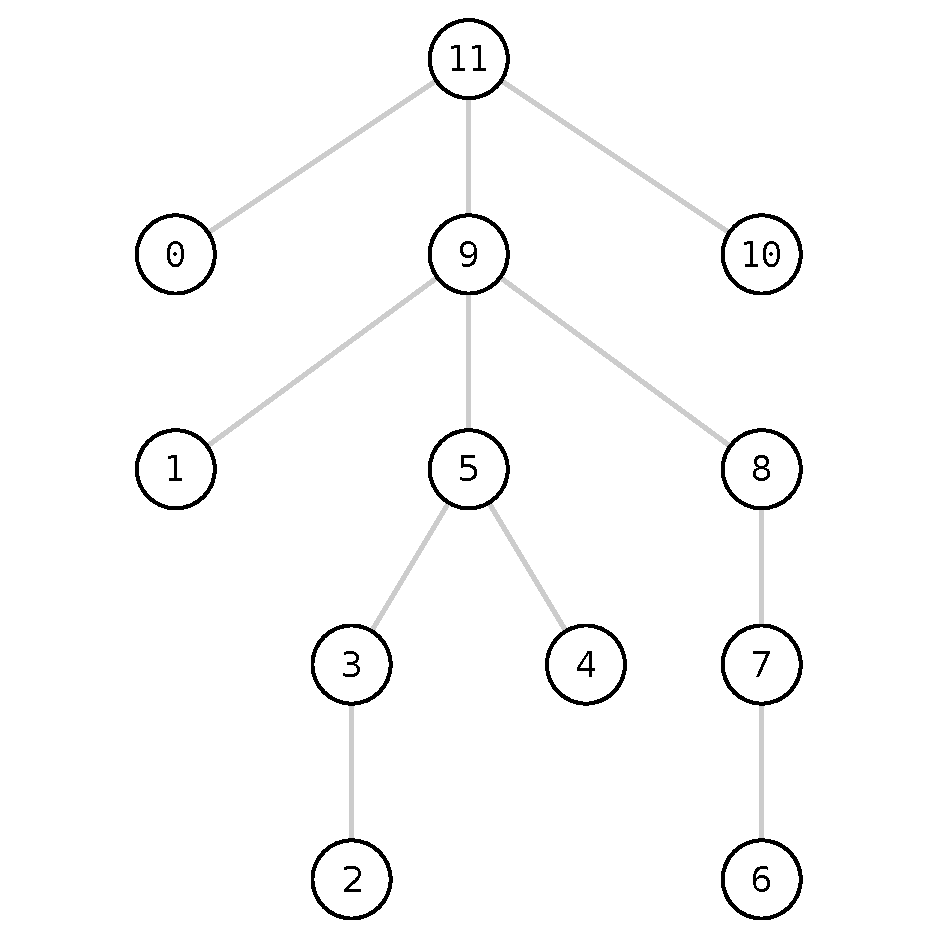
\includegraphics[width=0.28\textwidth]{python/lec02/dfs/dfs-0.pdf}\\[2pt]{\scriptsize Шаг 0}} &
\shortstack{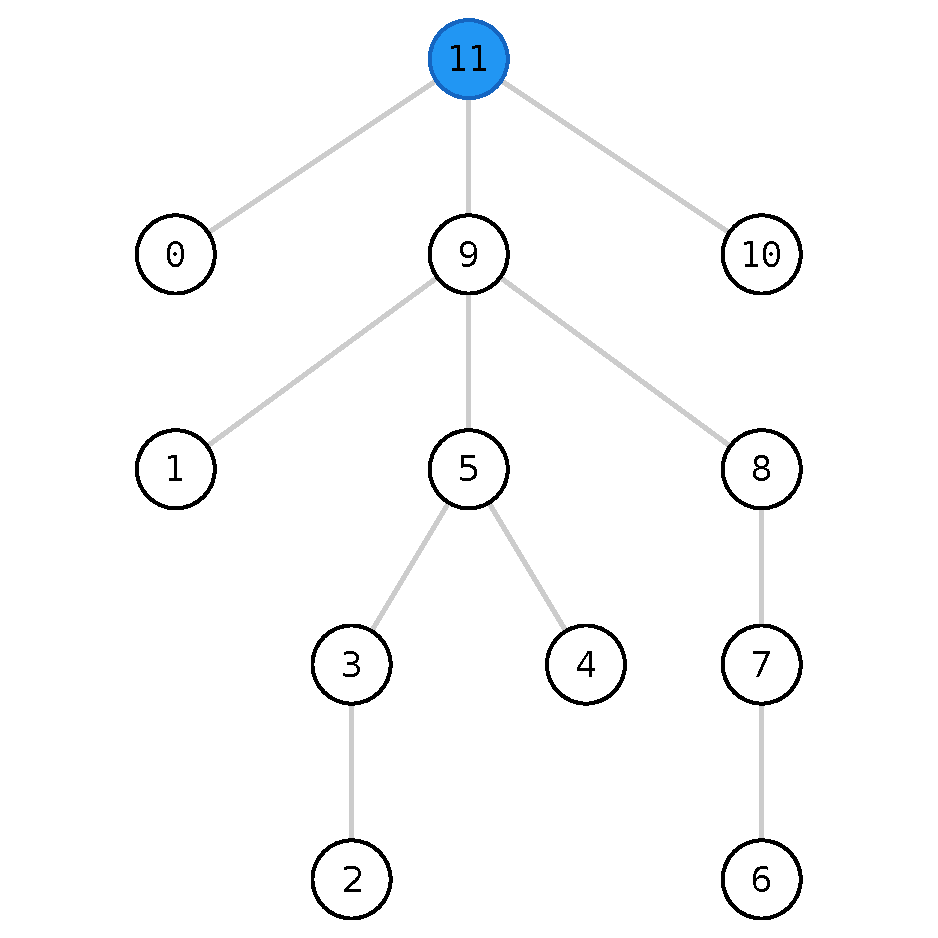
\includegraphics[width=0.28\textwidth]{python/lec02/dfs/dfs-1.pdf}\\[2pt]{\scriptsize Шаг 1}} &
\shortstack{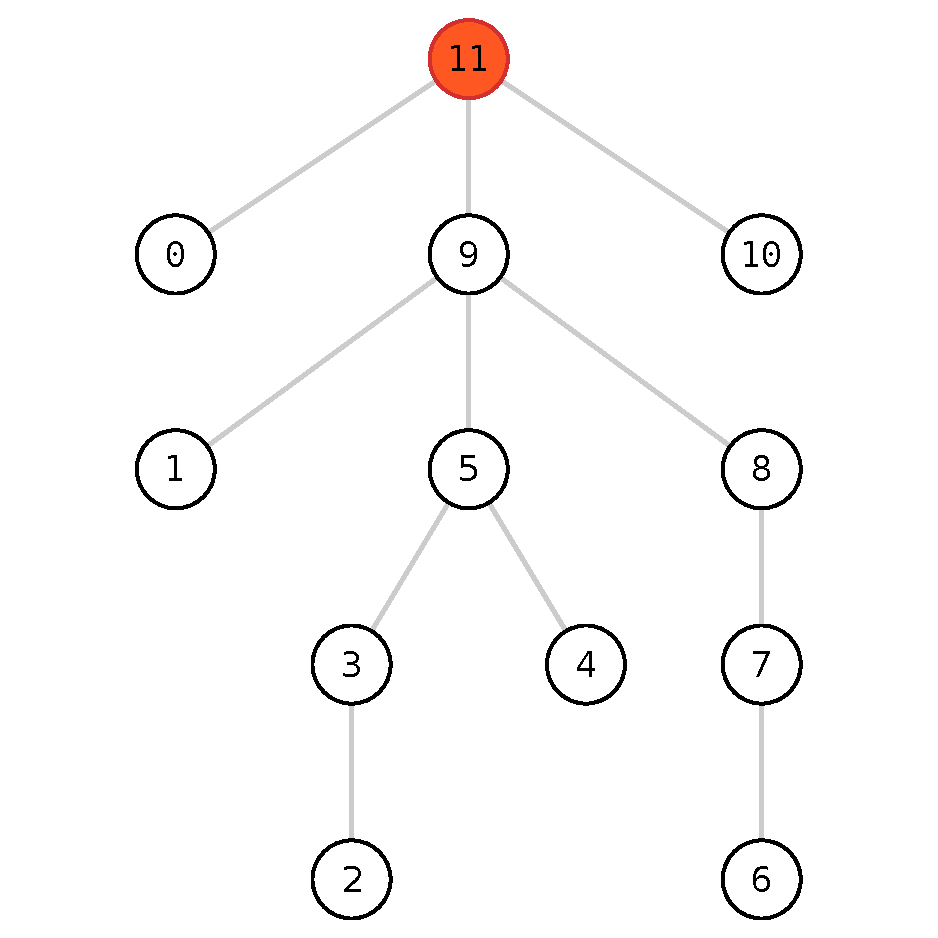
\includegraphics[width=0.28\textwidth]{python/lec02/dfs/dfs-2.pdf}\\[2pt]{\scriptsize Шаг 2}} \\
\end{tabular}\end{center}
\begin{center}\begin{tabular}{ccc}
\shortstack{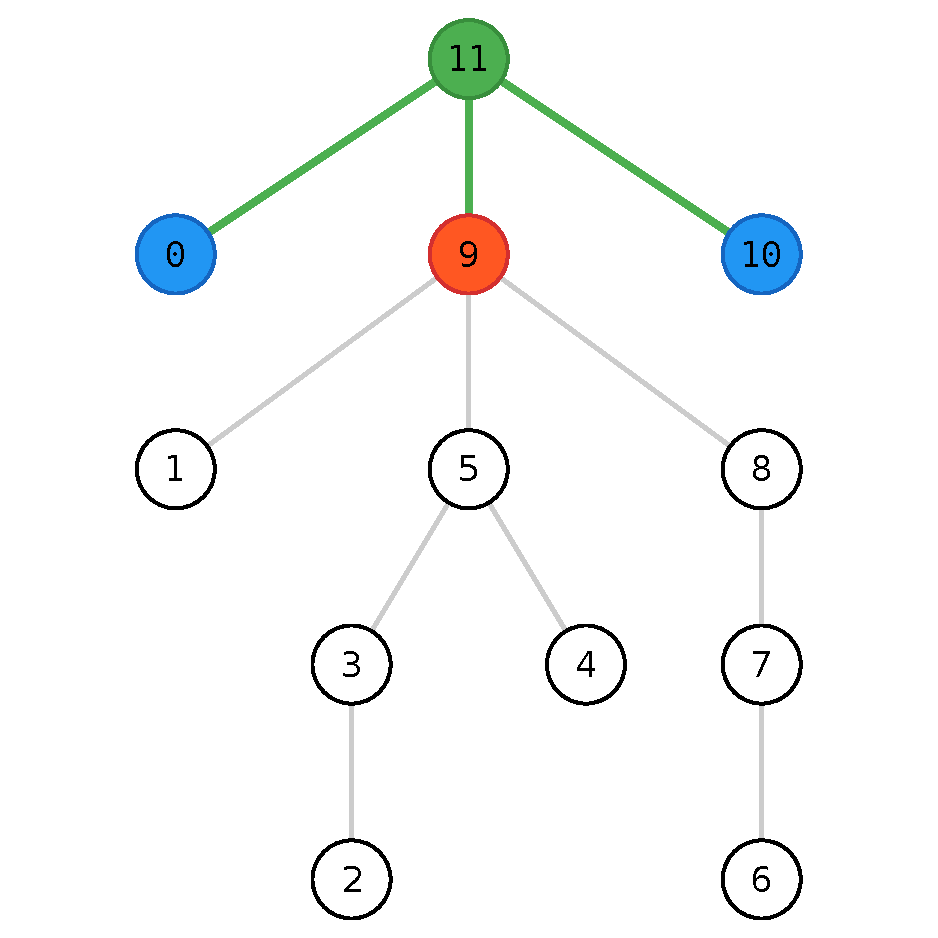
\includegraphics[width=0.28\textwidth]{python/lec02/dfs/dfs-3.pdf}\\[2pt]{\scriptsize Шаг 3}} &
\shortstack{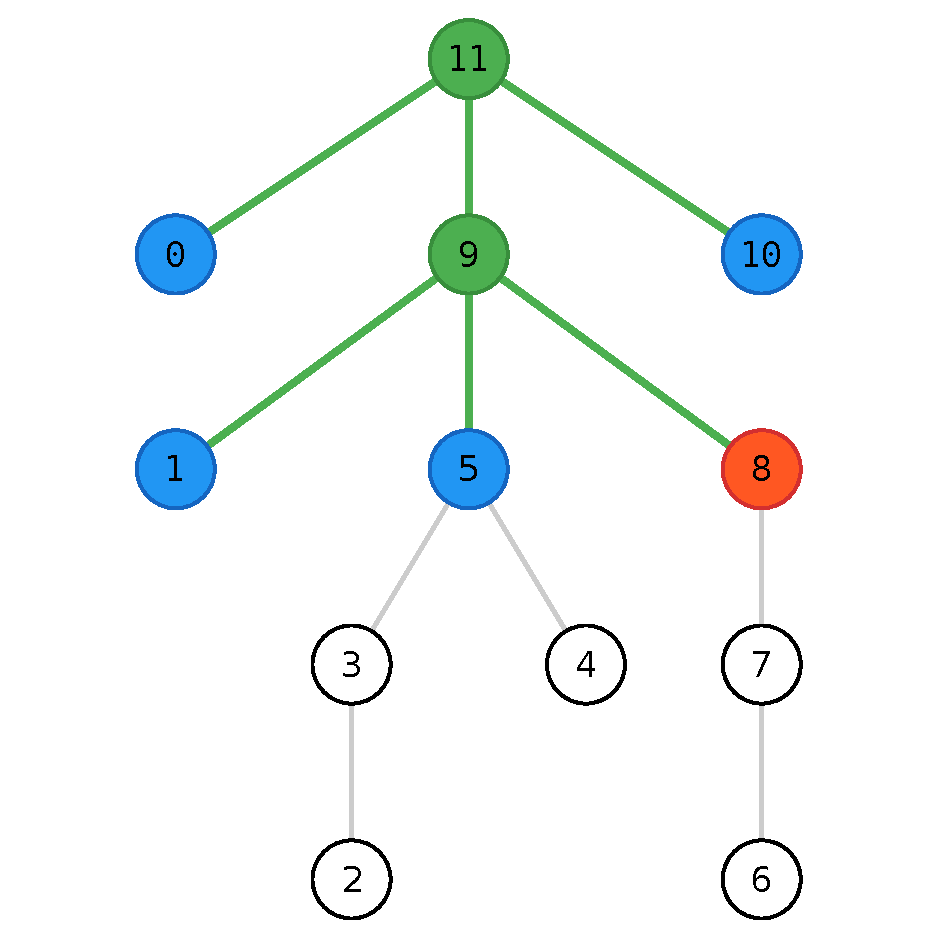
\includegraphics[width=0.28\textwidth]{python/lec02/dfs/dfs-4.pdf}\\[2pt]{\scriptsize Шаг 4}} &
\shortstack{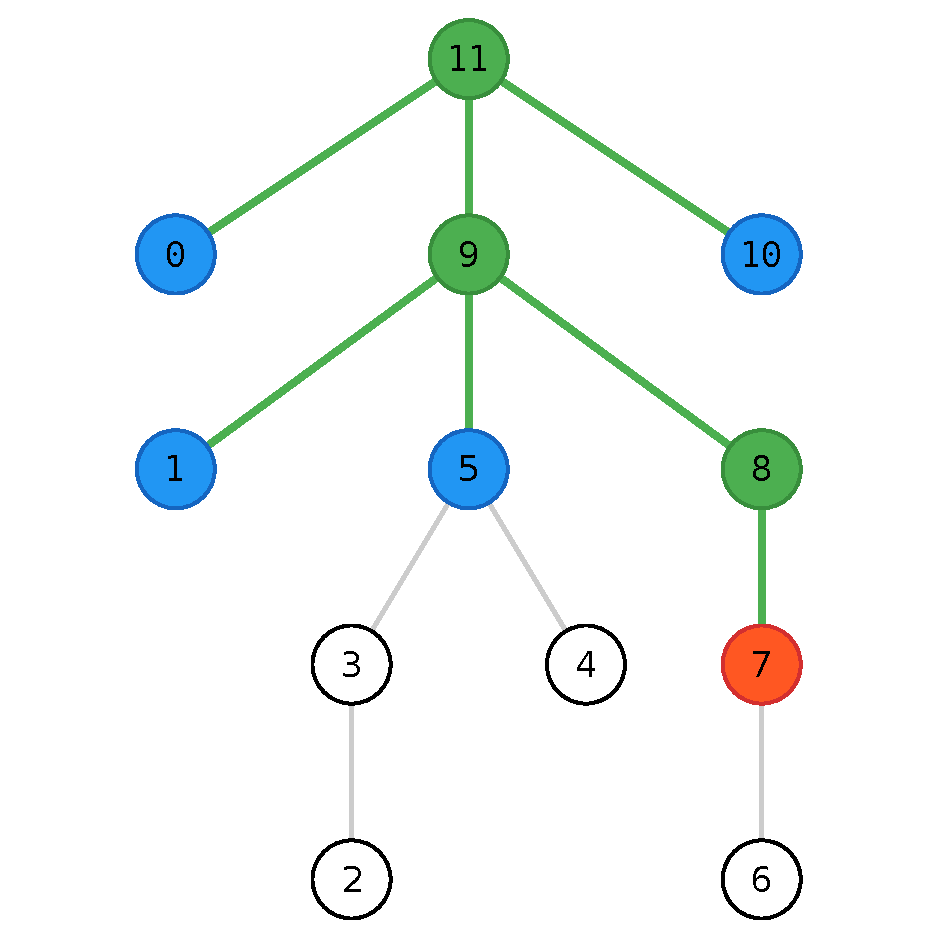
\includegraphics[width=0.28\textwidth]{python/lec02/dfs/dfs-5.pdf}\\[2pt]{\scriptsize Шаг 5}} \\
\end{tabular}\end{center}
\begin{center}\begin{tabular}{ccc}
\shortstack{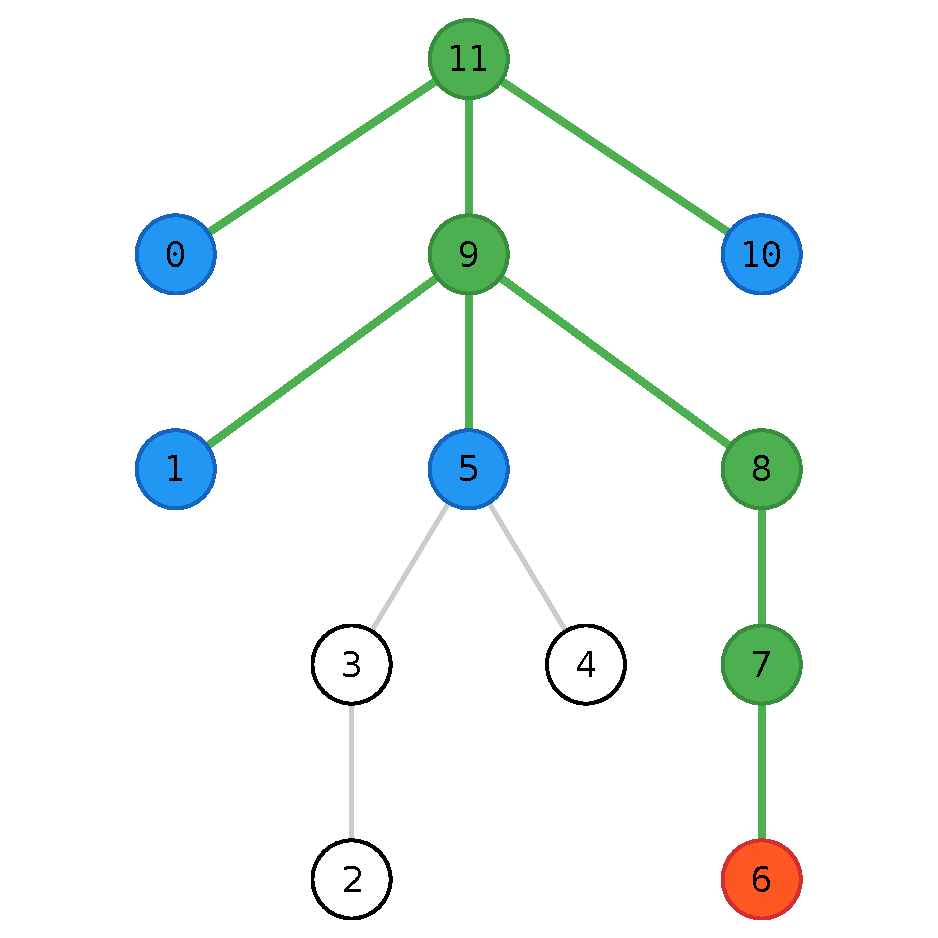
\includegraphics[width=0.28\textwidth]{python/lec02/dfs/dfs-6.pdf}\\[2pt]{\scriptsize Шаг 6}} &
\shortstack{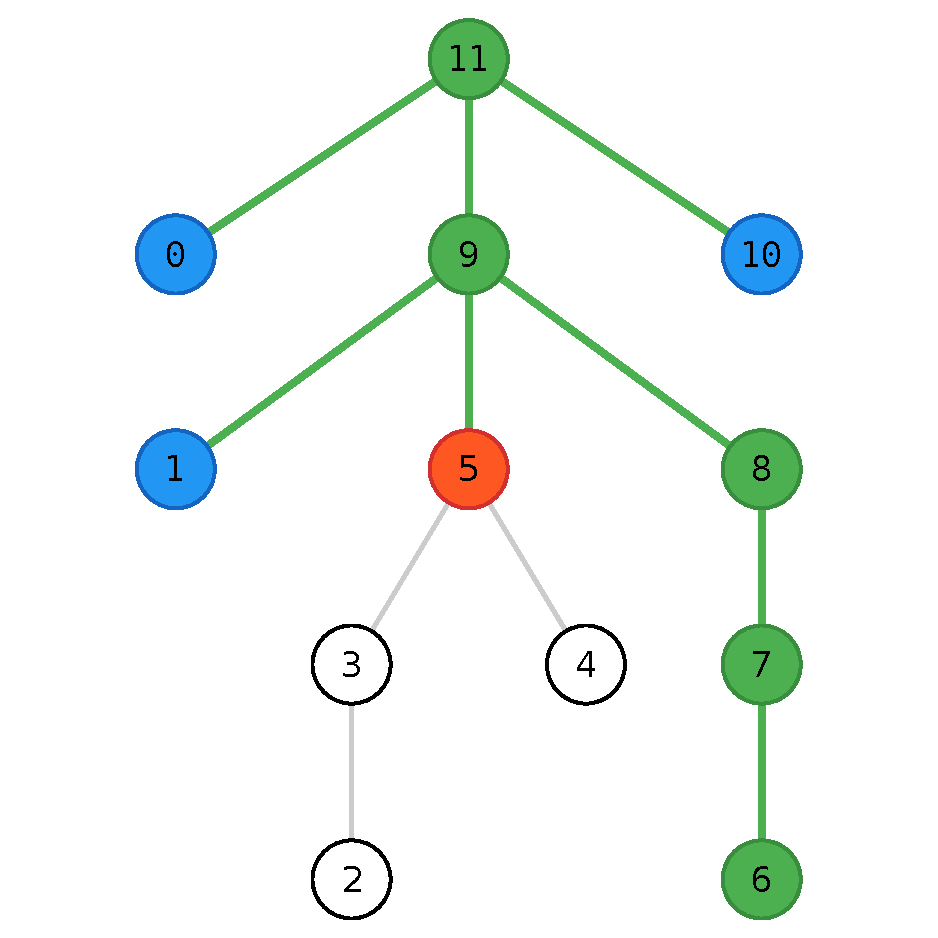
\includegraphics[width=0.28\textwidth]{python/lec02/dfs/dfs-7.pdf}\\[2pt]{\scriptsize Шаг 7}} &
\shortstack{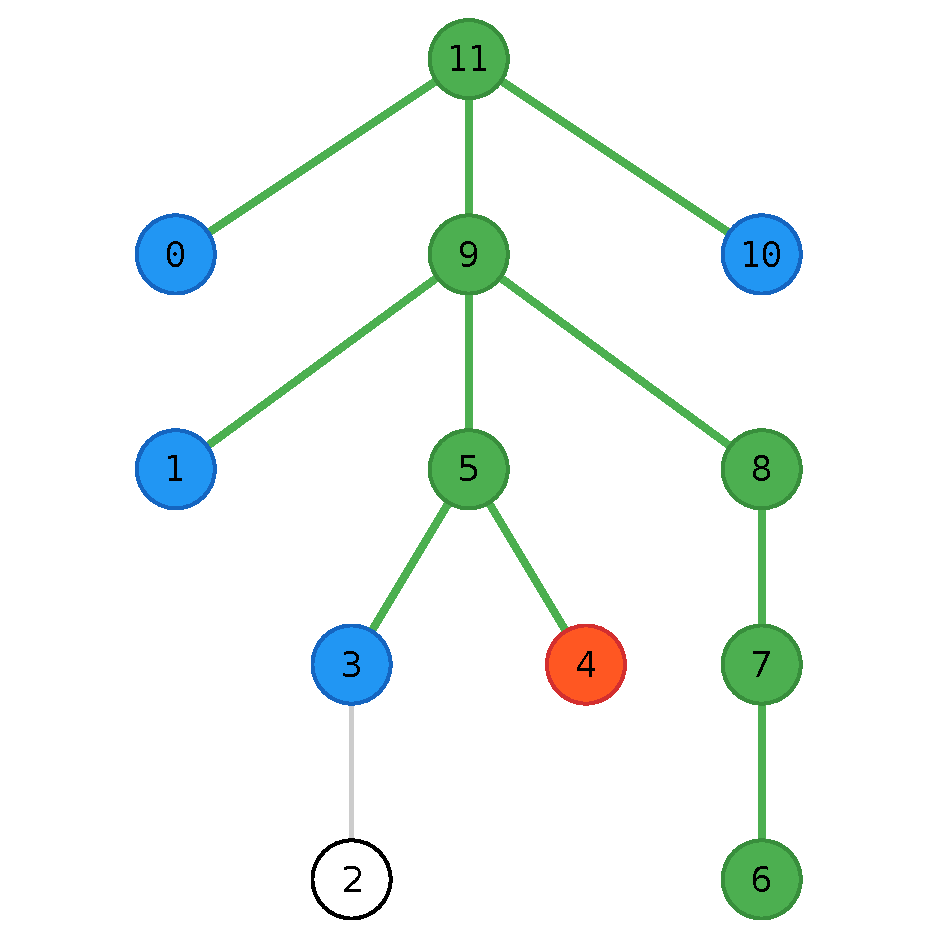
\includegraphics[width=0.28\textwidth]{python/lec02/dfs/dfs-8.pdf}\\[2pt]{\scriptsize Шаг 8}} \\
\end{tabular}\end{center}
\begin{center}\begin{tabular}{ccc}
\shortstack{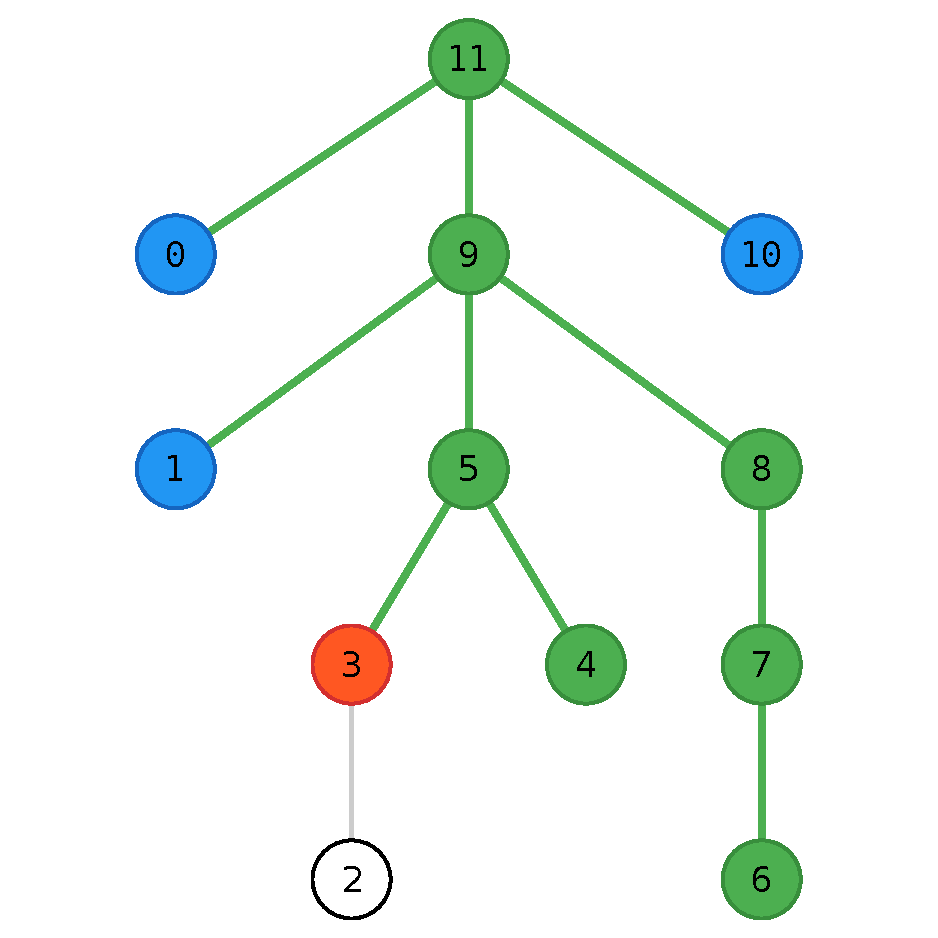
\includegraphics[width=0.28\textwidth]{python/lec02/dfs/dfs-9.pdf}\\[2pt]{\scriptsize Шаг 9}} &
\shortstack{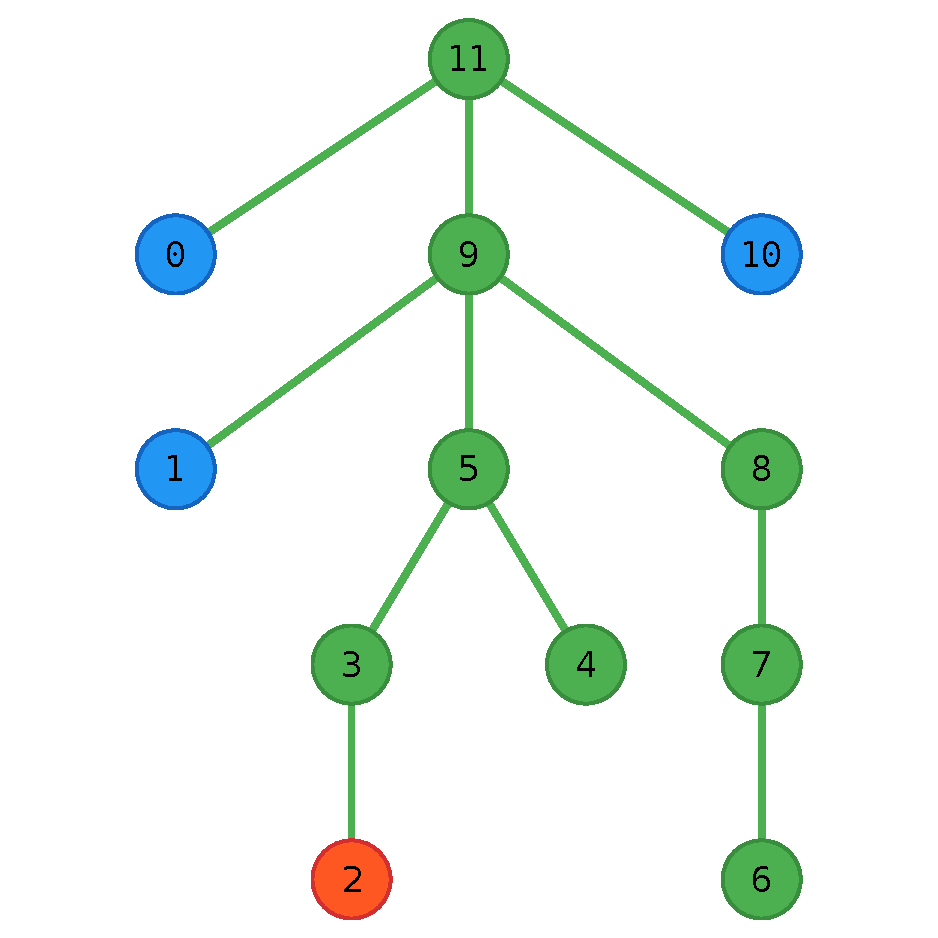
\includegraphics[width=0.28\textwidth]{python/lec02/dfs/dfs-10.pdf}\\[2pt]{\scriptsize Шаг 10}} &
\shortstack{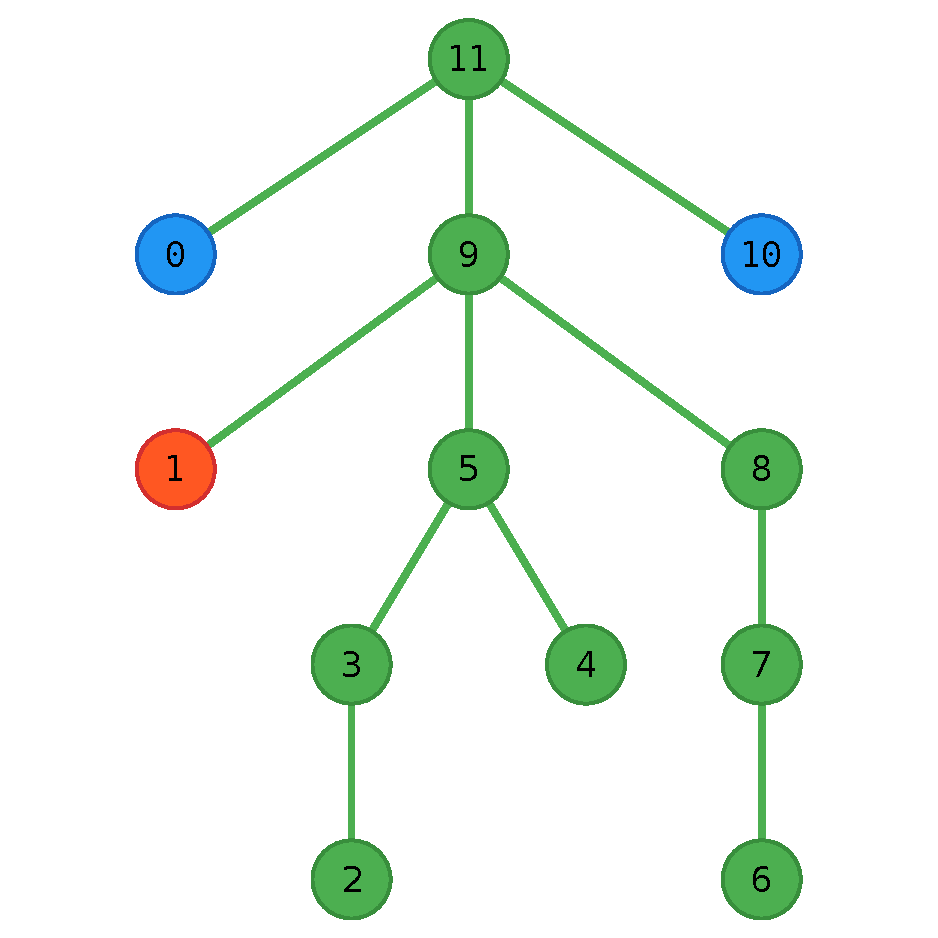
\includegraphics[width=0.28\textwidth]{python/lec02/dfs/dfs-11.pdf}\\[2pt]{\scriptsize Шаг 11}} \\
\end{tabular}\end{center}
\begin{center}\begin{tabular}{ccc}
\shortstack{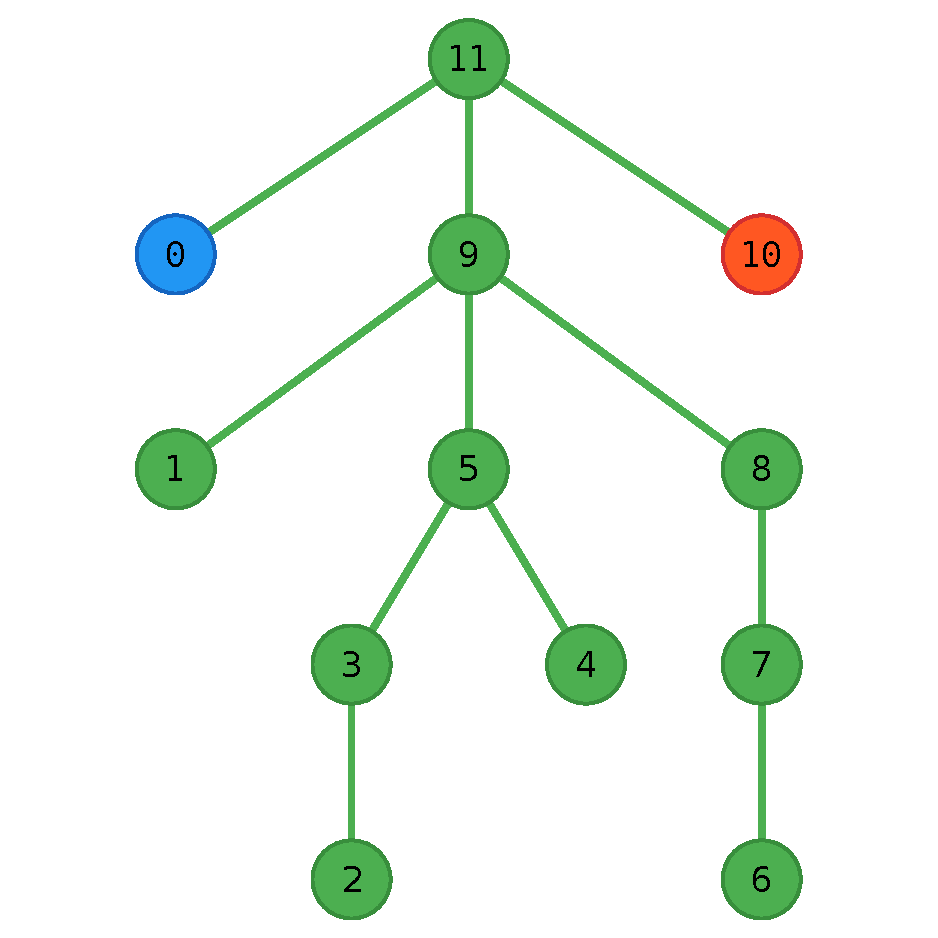
\includegraphics[width=0.28\textwidth]{python/lec02/dfs/dfs-12.pdf}\\[2pt]{\scriptsize Шаг 12}} &
\shortstack{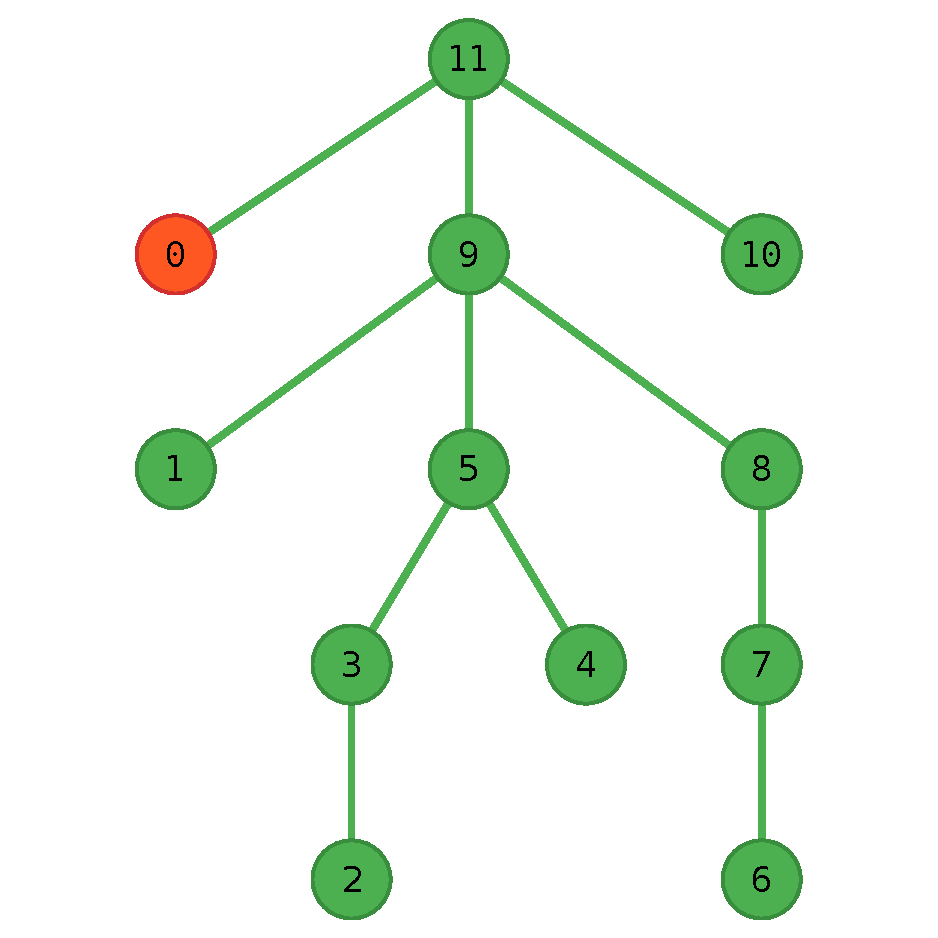
\includegraphics[width=0.28\textwidth]{python/lec02/dfs/dfs-13.pdf}\\[2pt]{\scriptsize Шаг 13}} &
\shortstack{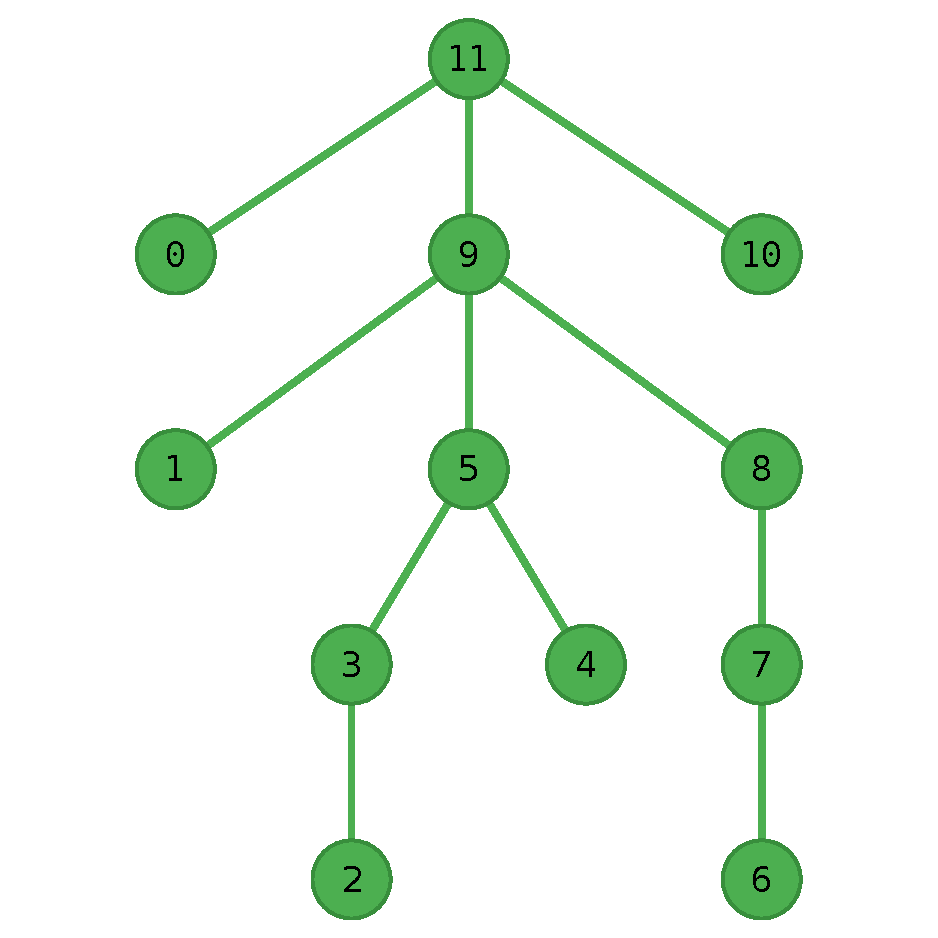
\includegraphics[width=0.28\textwidth]{python/lec02/dfs/dfs-14.pdf}\\[2pt]{\scriptsize Шаг 14}} \\
\end{tabular}\end{center}

\noindent\textbf{Пример работы BFS} (старт из $S$):

\begin{center}\begin{tabular}{ccc}
\shortstack{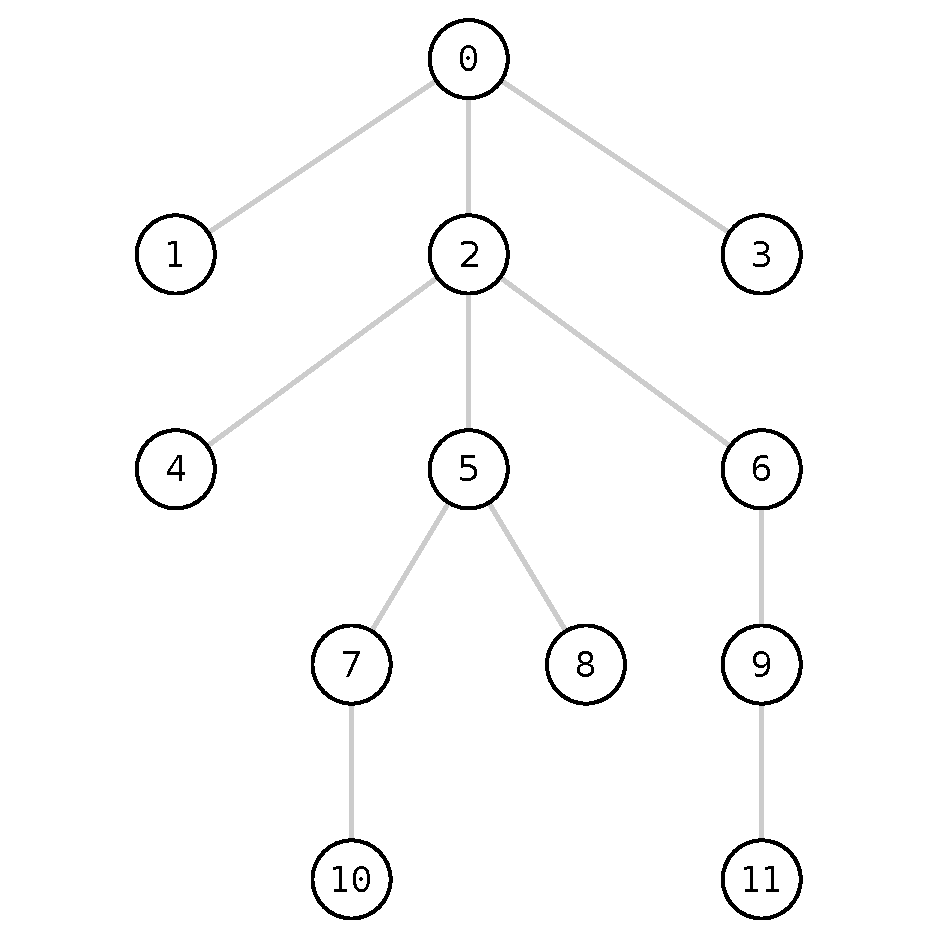
\includegraphics[width=0.28\textwidth]{python/lec02/bfs/bfs-0.pdf}\\[2pt]{\scriptsize Шаг 0}} &
\shortstack{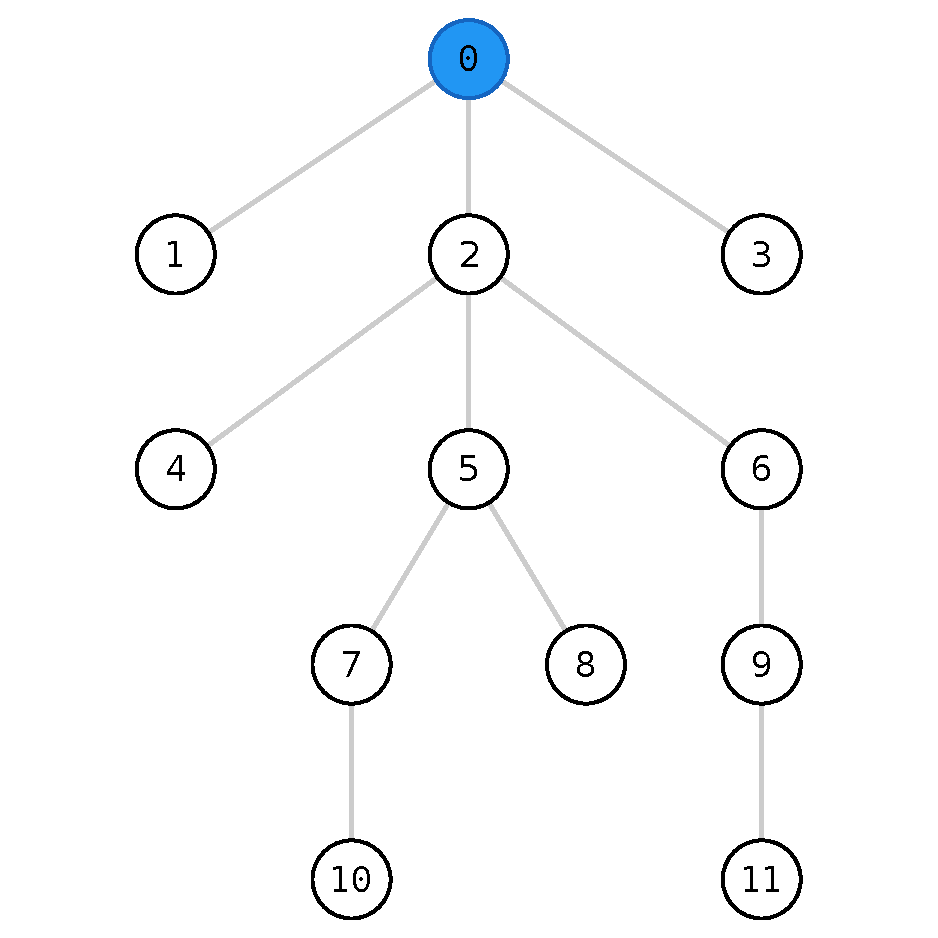
\includegraphics[width=0.28\textwidth]{python/lec02/bfs/bfs-1.pdf}\\[2pt]{\scriptsize Шаг 1}} &
\shortstack{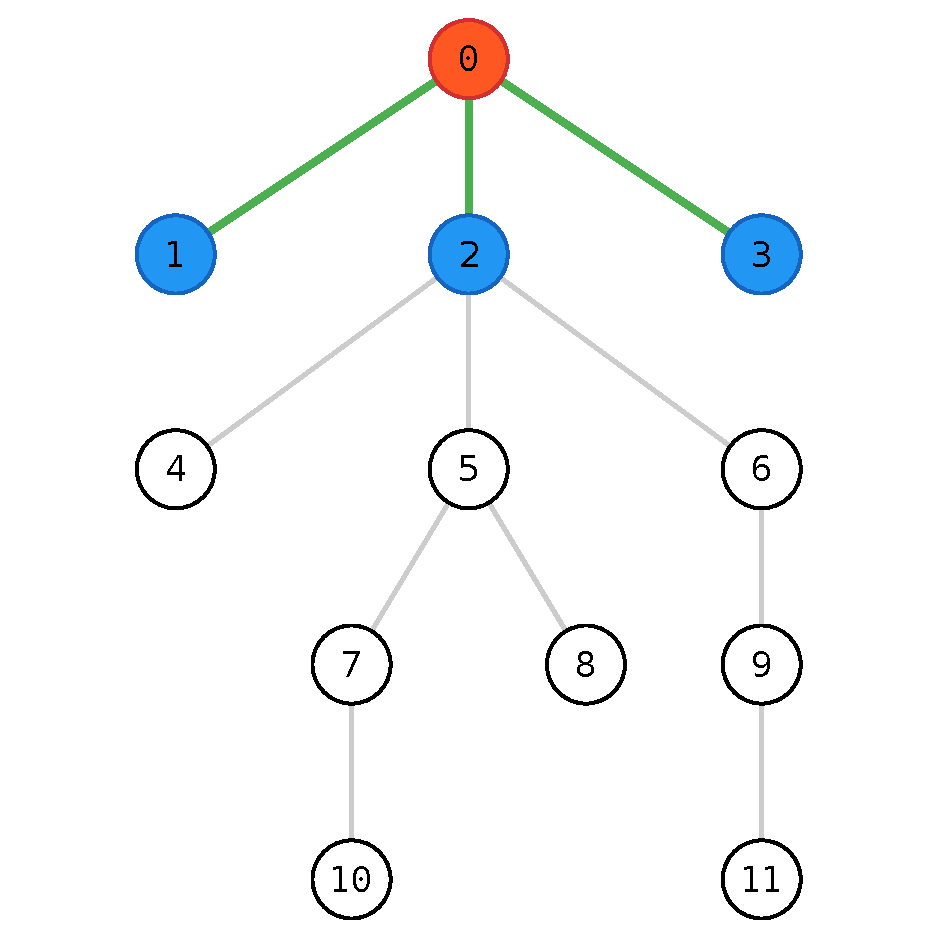
\includegraphics[width=0.28\textwidth]{python/lec02/bfs/bfs-2.pdf}\\[2pt]{\scriptsize Шаг 2}} \\
\end{tabular}\end{center}
\begin{center}\begin{tabular}{ccc}
\shortstack{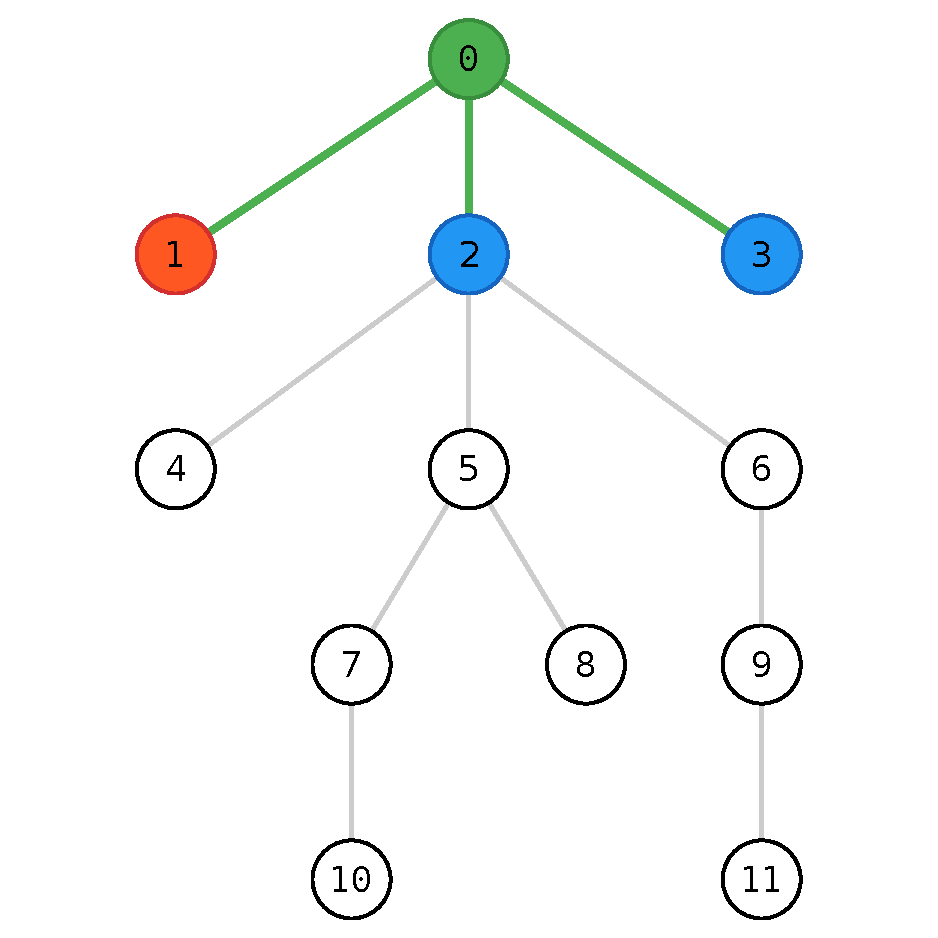
\includegraphics[width=0.28\textwidth]{python/lec02/bfs/bfs-3.pdf}\\[2pt]{\scriptsize Шаг 3}} &
\shortstack{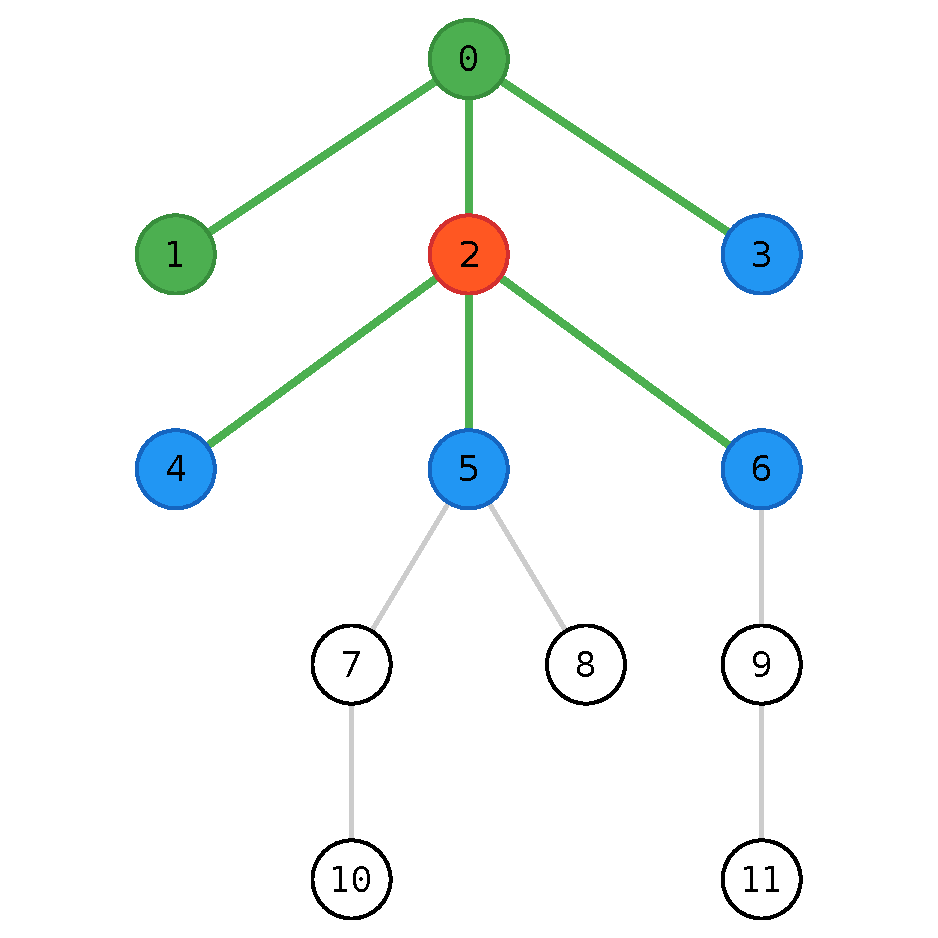
\includegraphics[width=0.28\textwidth]{python/lec02/bfs/bfs-4.pdf}\\[2pt]{\scriptsize Шаг 4}} &
\shortstack{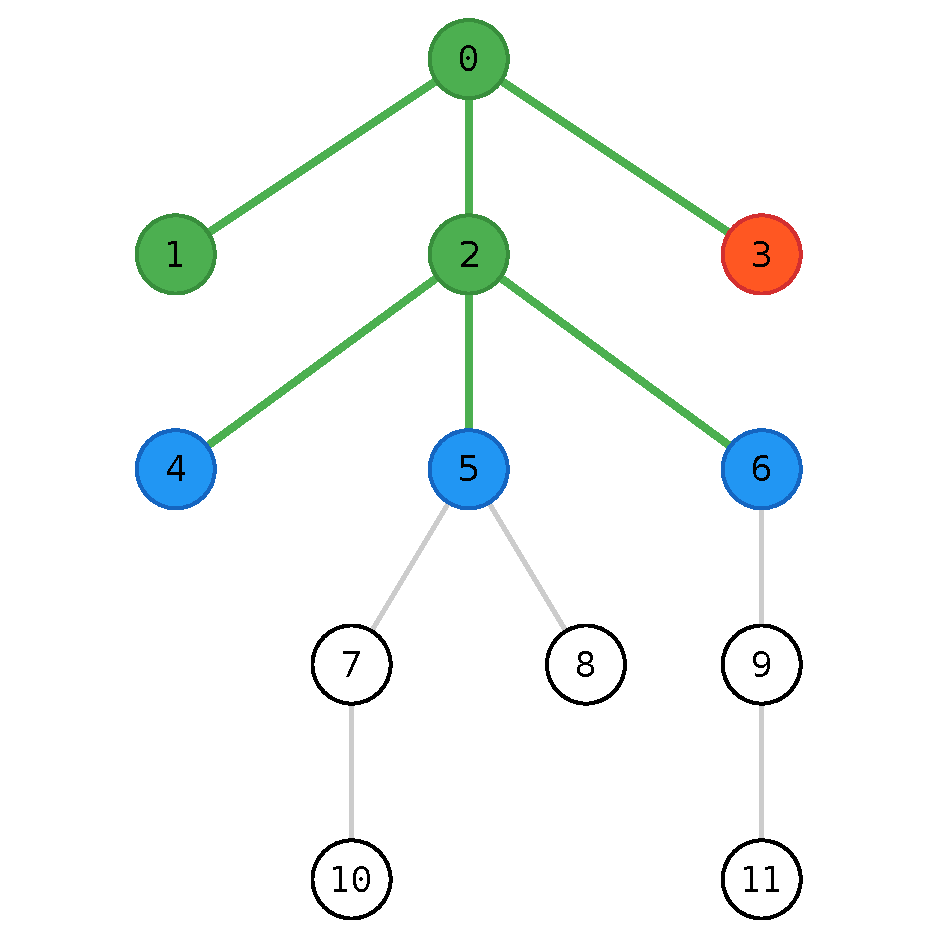
\includegraphics[width=0.28\textwidth]{python/lec02/bfs/bfs-5.pdf}\\[2pt]{\scriptsize Шаг 5}} \\
\end{tabular}\end{center}
\begin{center}\begin{tabular}{ccc}
\shortstack{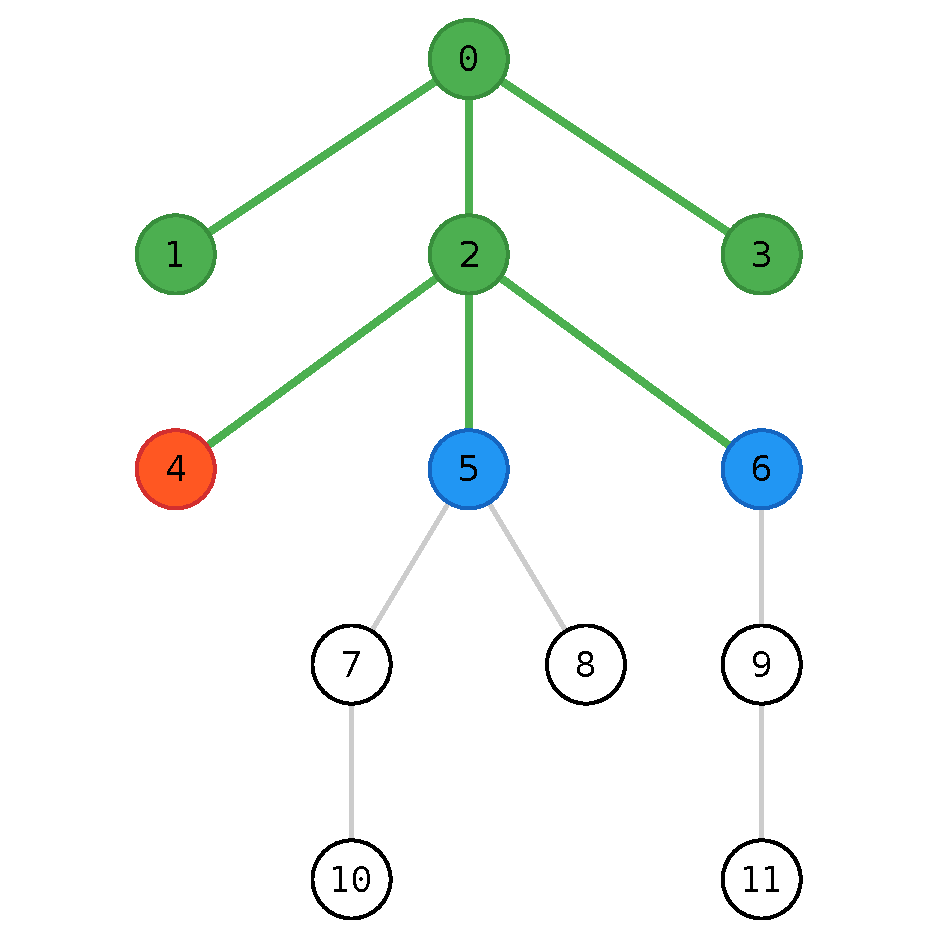
\includegraphics[width=0.28\textwidth]{python/lec02/bfs/bfs-6.pdf}\\[2pt]{\scriptsize Шаг 6}} &
\shortstack{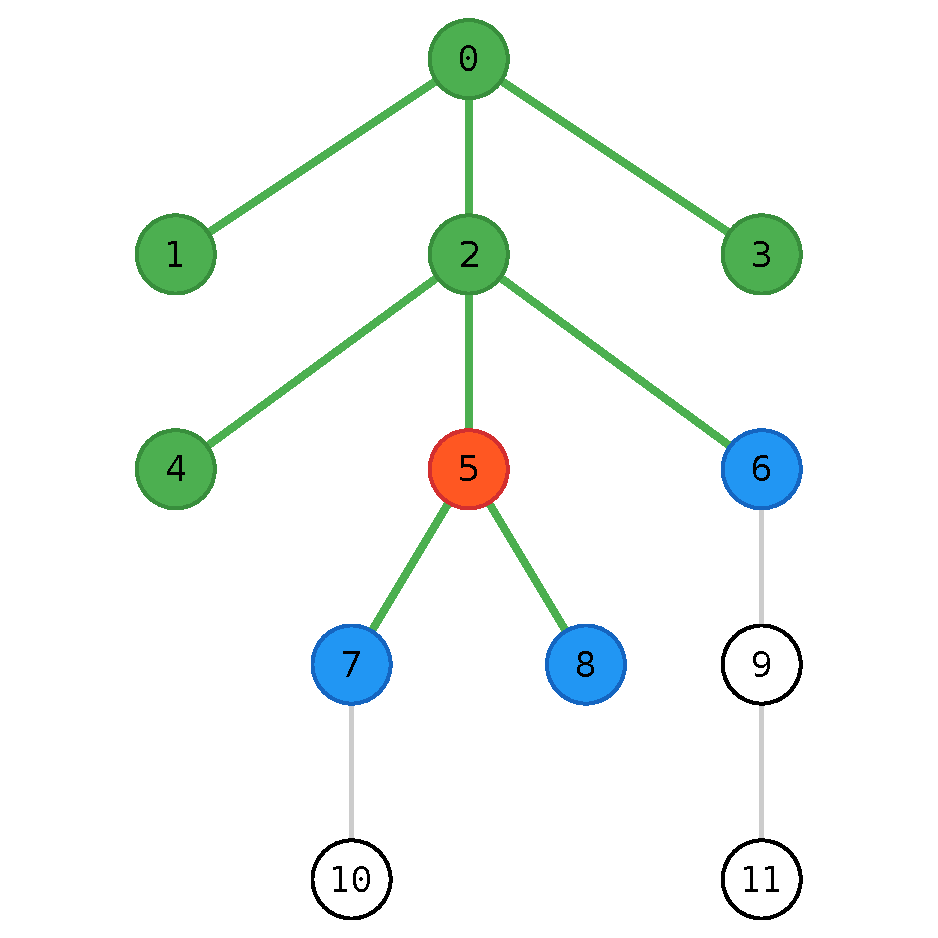
\includegraphics[width=0.28\textwidth]{python/lec02/bfs/bfs-7.pdf}\\[2pt]{\scriptsize Шаг 7}} &
\shortstack{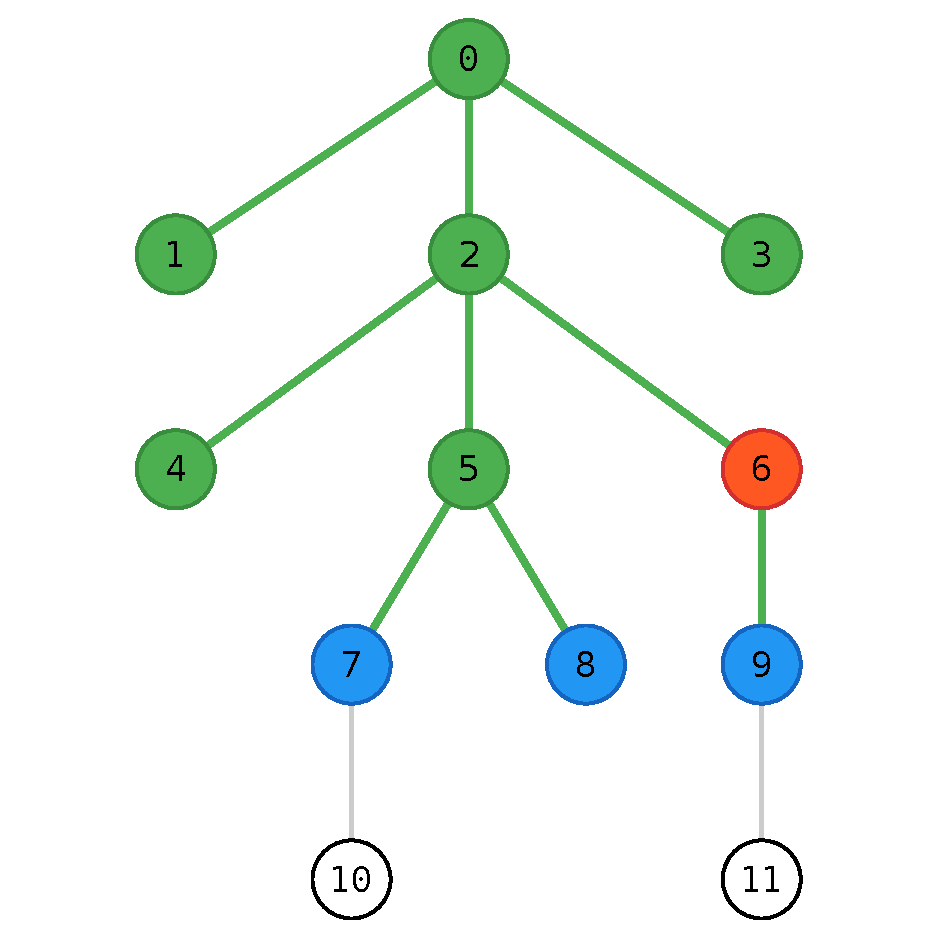
\includegraphics[width=0.28\textwidth]{python/lec02/bfs/bfs-8.pdf}\\[2pt]{\scriptsize Шаг 8}} \\
\end{tabular}\end{center}
\begin{center}\begin{tabular}{ccc}
\shortstack{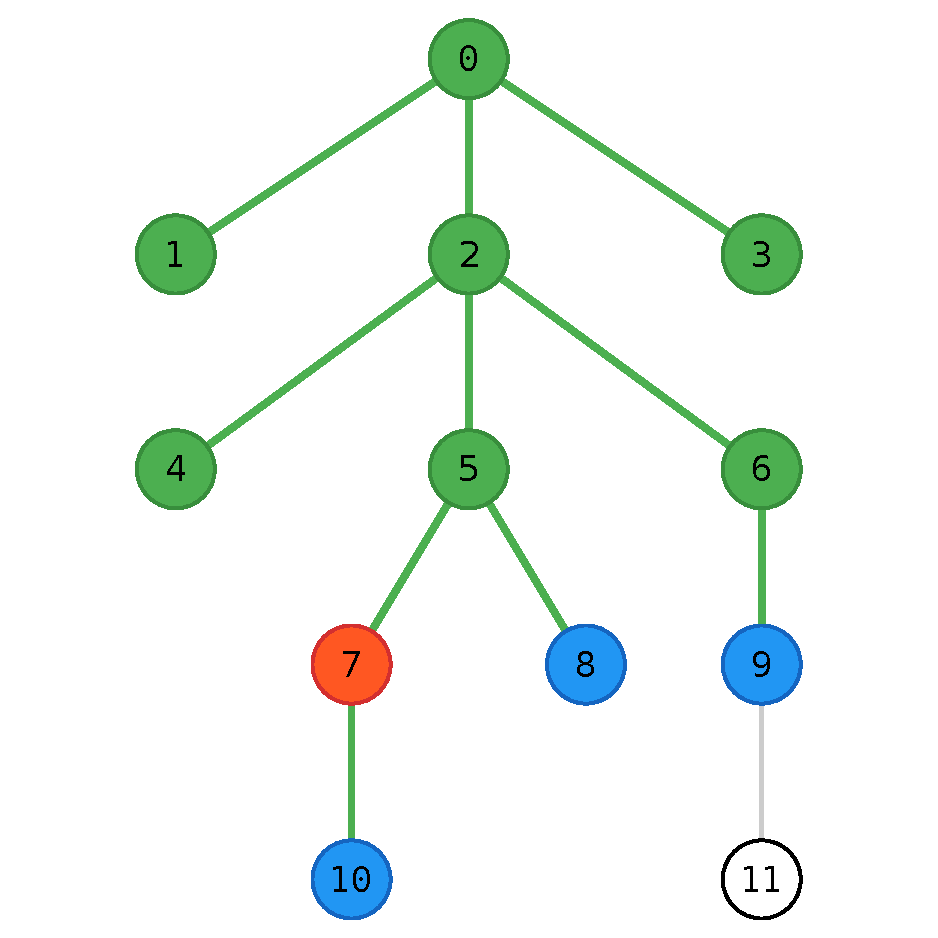
\includegraphics[width=0.28\textwidth]{python/lec02/bfs/bfs-9.pdf}\\[2pt]{\scriptsize Шаг 9}} &
\shortstack{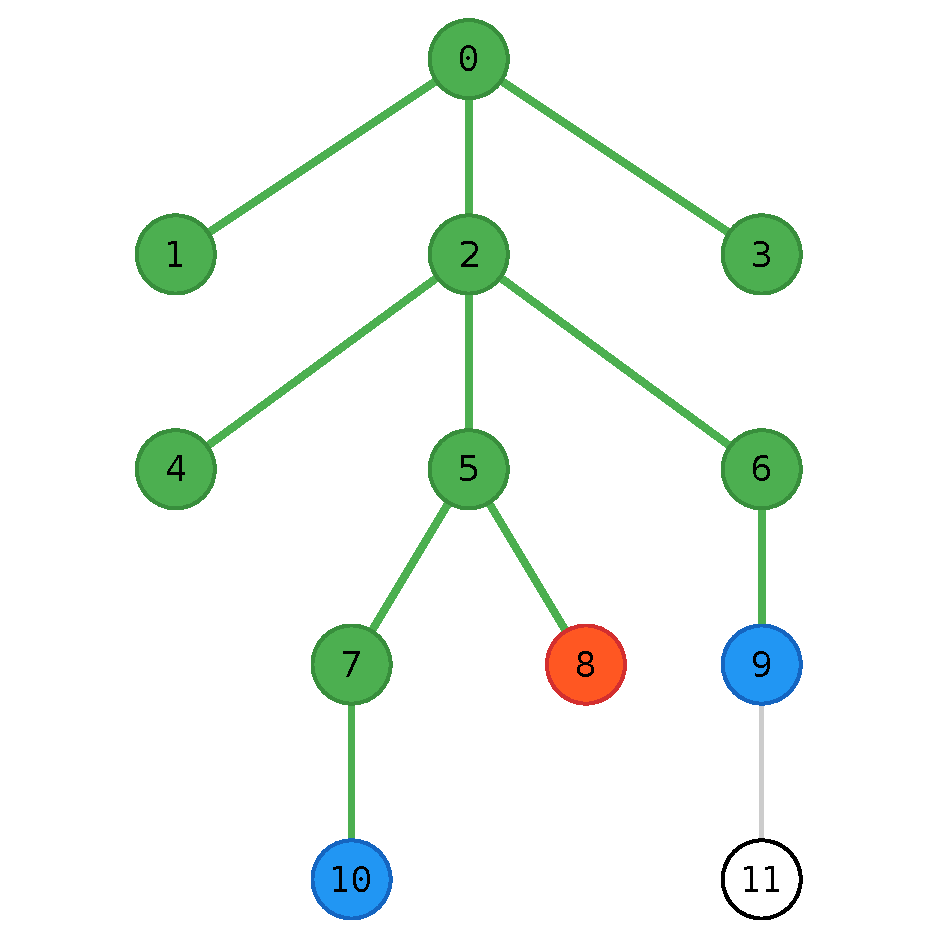
\includegraphics[width=0.28\textwidth]{python/lec02/bfs/bfs-10.pdf}\\[2pt]{\scriptsize Шаг 10}} &
\shortstack{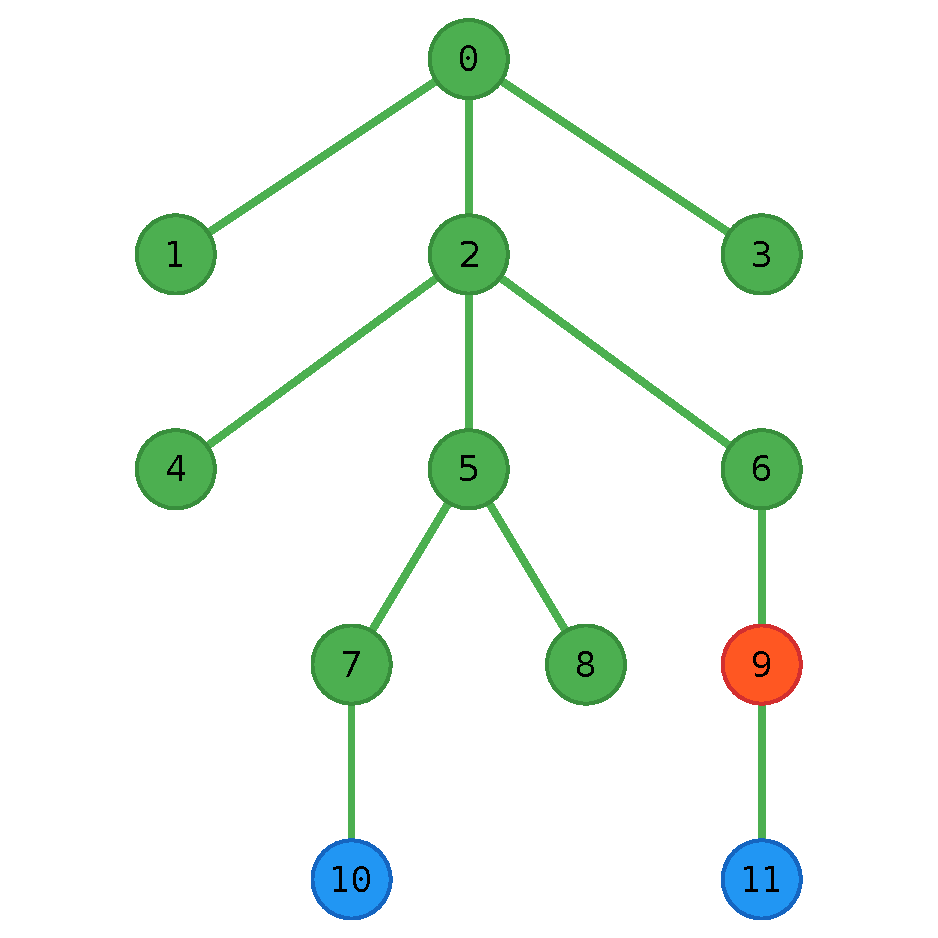
\includegraphics[width=0.28\textwidth]{python/lec02/bfs/bfs-11.pdf}\\[2pt]{\scriptsize Шаг 11}} \\
\end{tabular}\end{center}
\begin{center}\begin{tabular}{ccc}
\shortstack{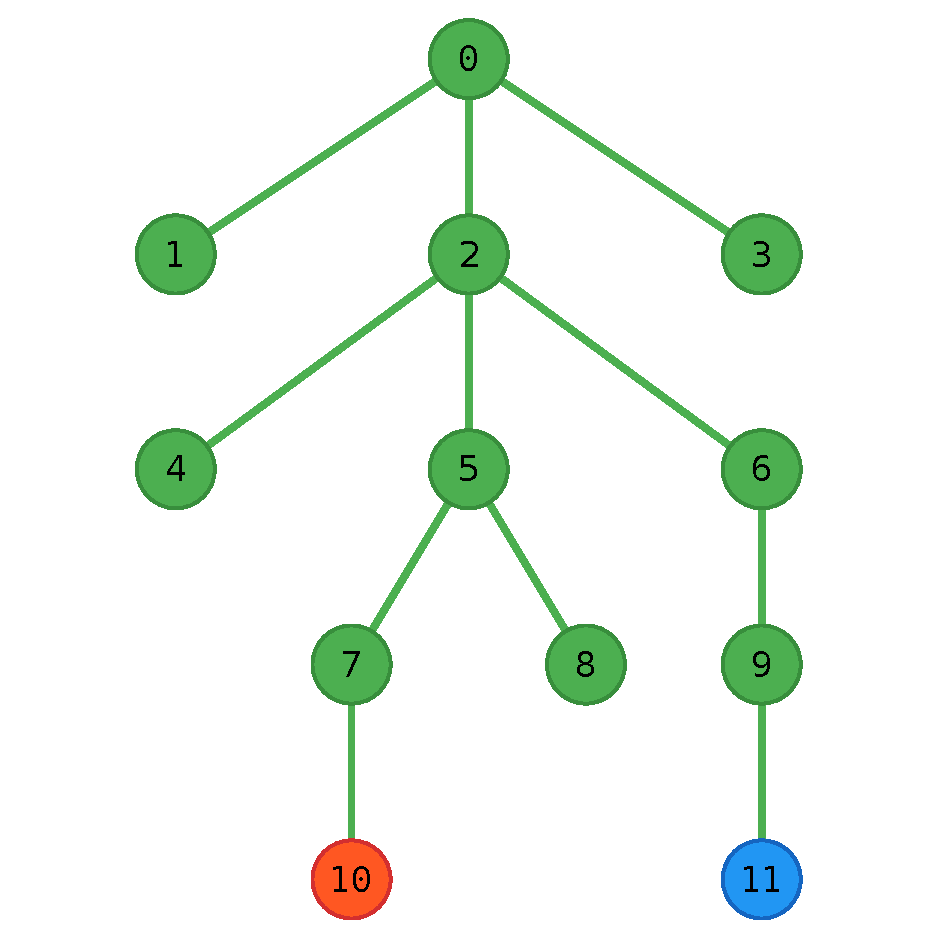
\includegraphics[width=0.28\textwidth]{python/lec02/bfs/bfs-12.pdf}\\[2pt]{\scriptsize Шаг 12}} &
\shortstack{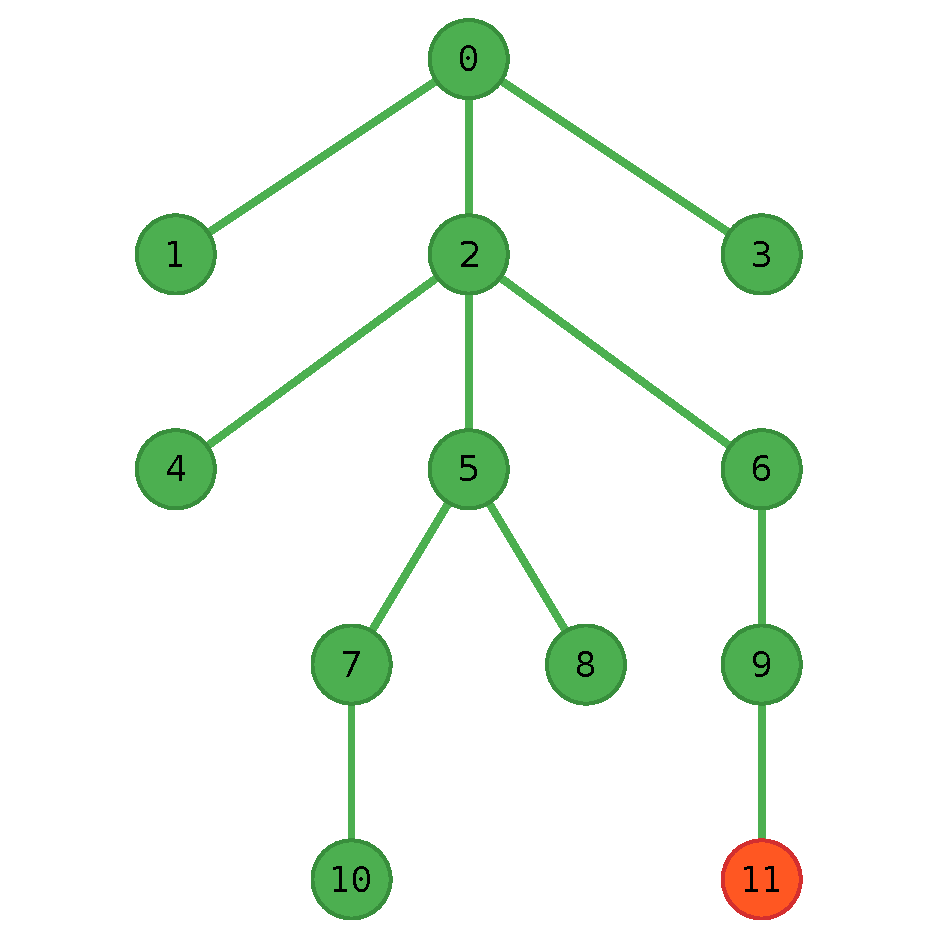
\includegraphics[width=0.28\textwidth]{python/lec02/bfs/bfs-13.pdf}\\[2pt]{\scriptsize Шаг 13}} &
\shortstack{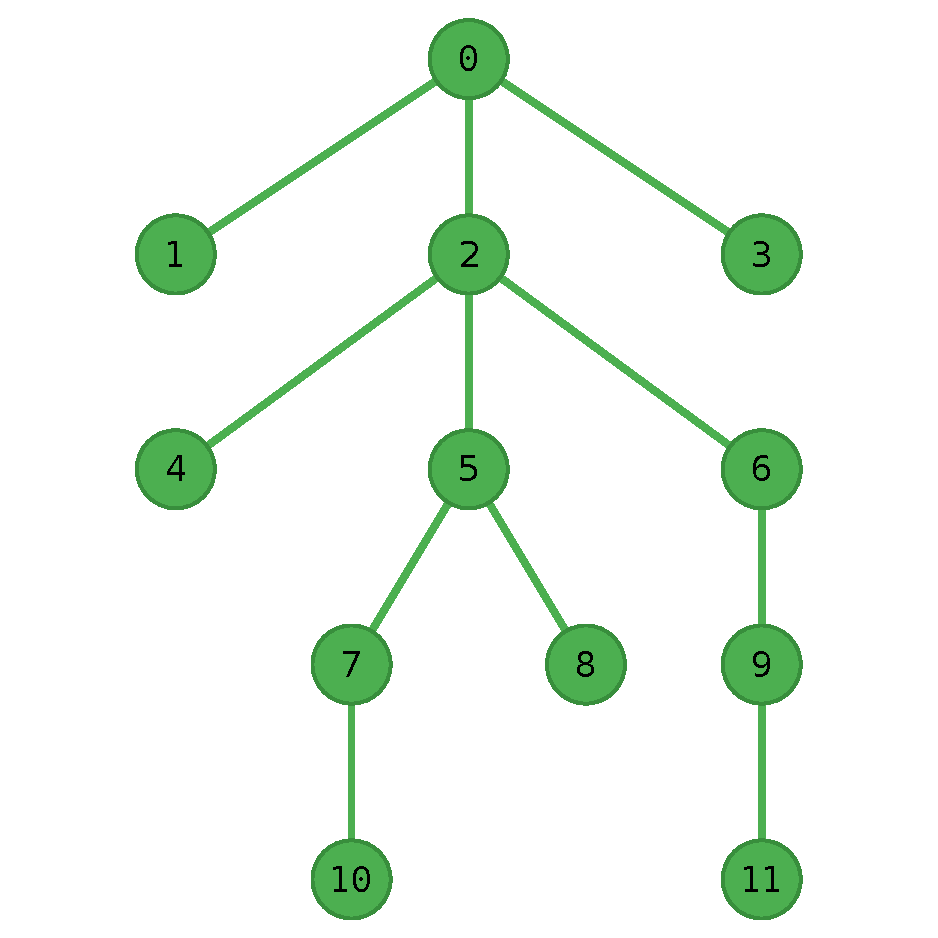
\includegraphics[width=0.28\textwidth]{python/lec02/bfs/bfs-14.pdf}\\[2pt]{\scriptsize Шаг 14}} \\
\end{tabular}\end{center}

\end{algo}


\bigskip
\begin{algo}{Топологическая сортировка (Topsort)}{topsort}
\textit{Дано:} ориентированный граф без циклов, задающий частичный порядок.
\textit{Построить:} линейный порядок, согласованный с исходным.

\medskip
\textbf{Шаг I.} Серия поисков в глубину (DFS). Когда вершина становится
<<тупиковой>> (все её исходящие рёбра уже обработаны), она кладётся в стек.

\textbf{Шаг II.} Нумеруем вершины по стеку \emph{снизу вверх}: самая нижняя
вершина стека получает номер~1, верхняя --- номер $n$. После этого
дорисовываем рефлексивные петли и недостающие рёбра: из каждой вершины
с \emph{бóльшим} номером --- во все вершины с \emph{меньшим} номером.

Результат --- граф, задающий отношение \textbf{линейного порядка}.

\medskip
\noindent\textbf{Работа алгоритма по шагам.} Исходный граф:

\begin{center}
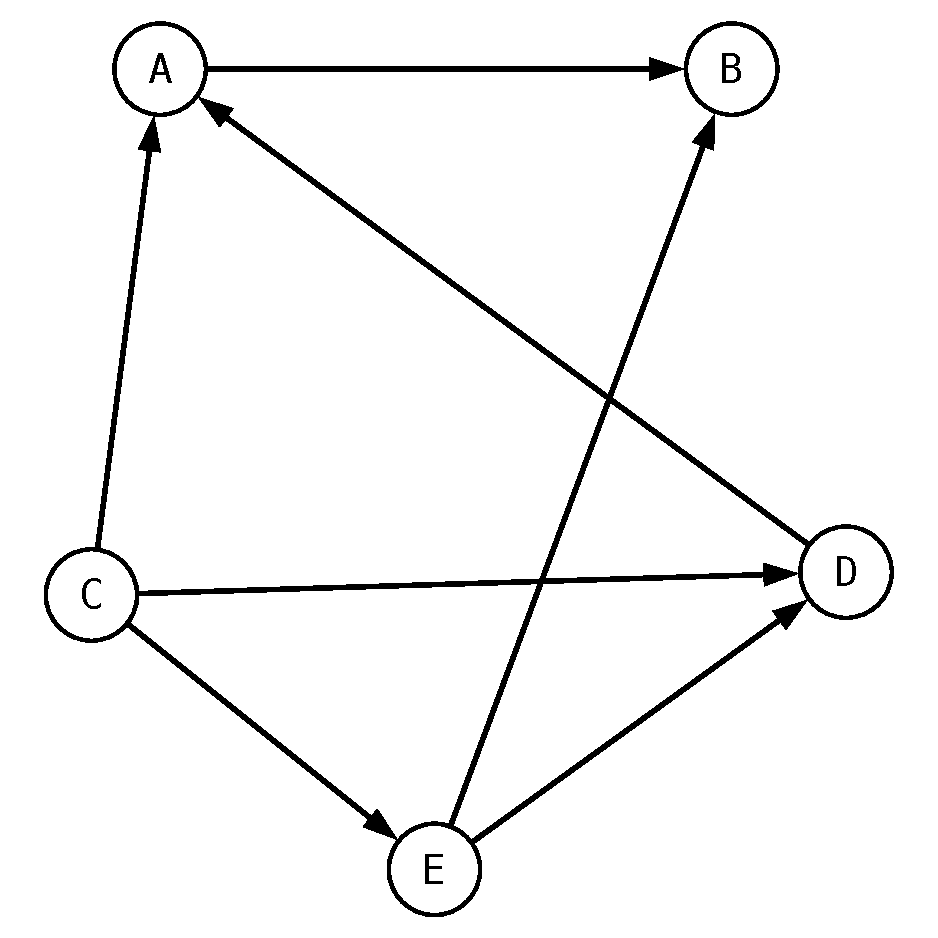
\includegraphics[width=0.5\textwidth]{figures/topsort-initial.pdf}
\end{center}

\noindent Активная ветка DFS --- синяя, текущая вершина --- оранжевая,
тупиковые (уложенные в стек) --- зелёные, рёбра дерева обхода --- зелёные.
Стек показан справа (верх стека --- сверху).

\begin{center}\begin{tabular}{ccc}
\shortstack{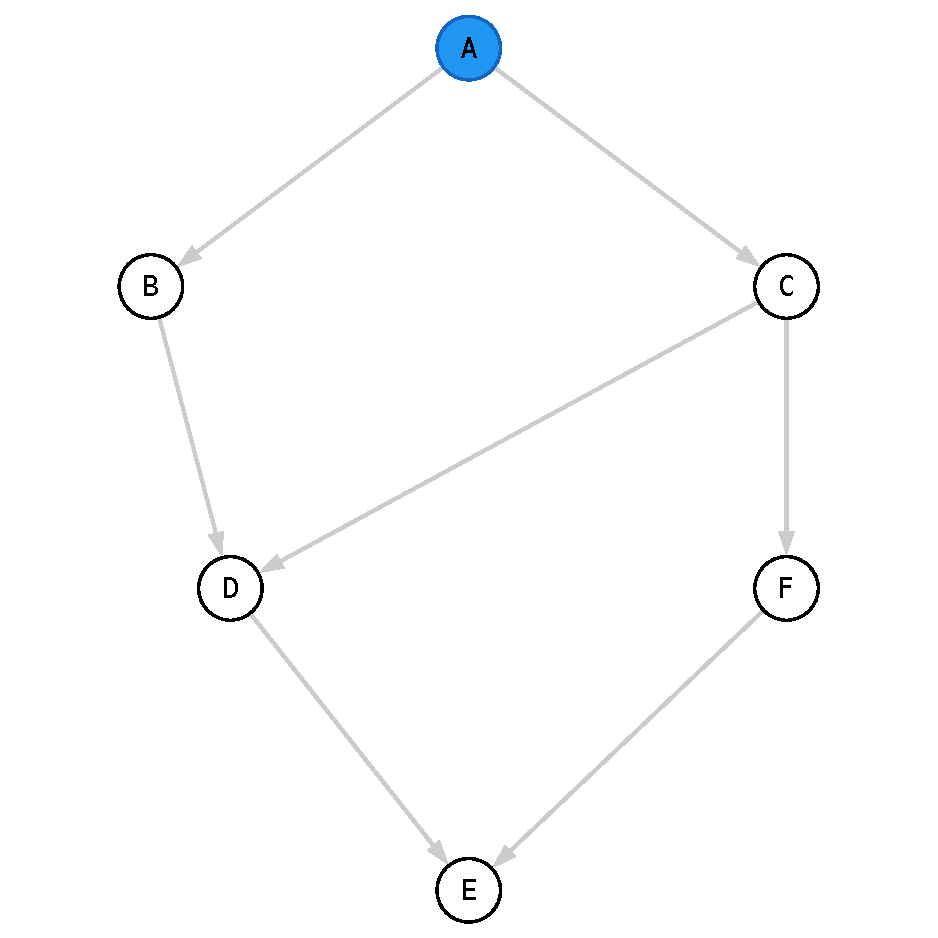
\includegraphics[width=0.30\textwidth]{python/lec02/topsort/topsort-0.pdf}\\[2pt]{\scriptsize Шаг 0. Исходный граф, стек пуст}} &
\shortstack{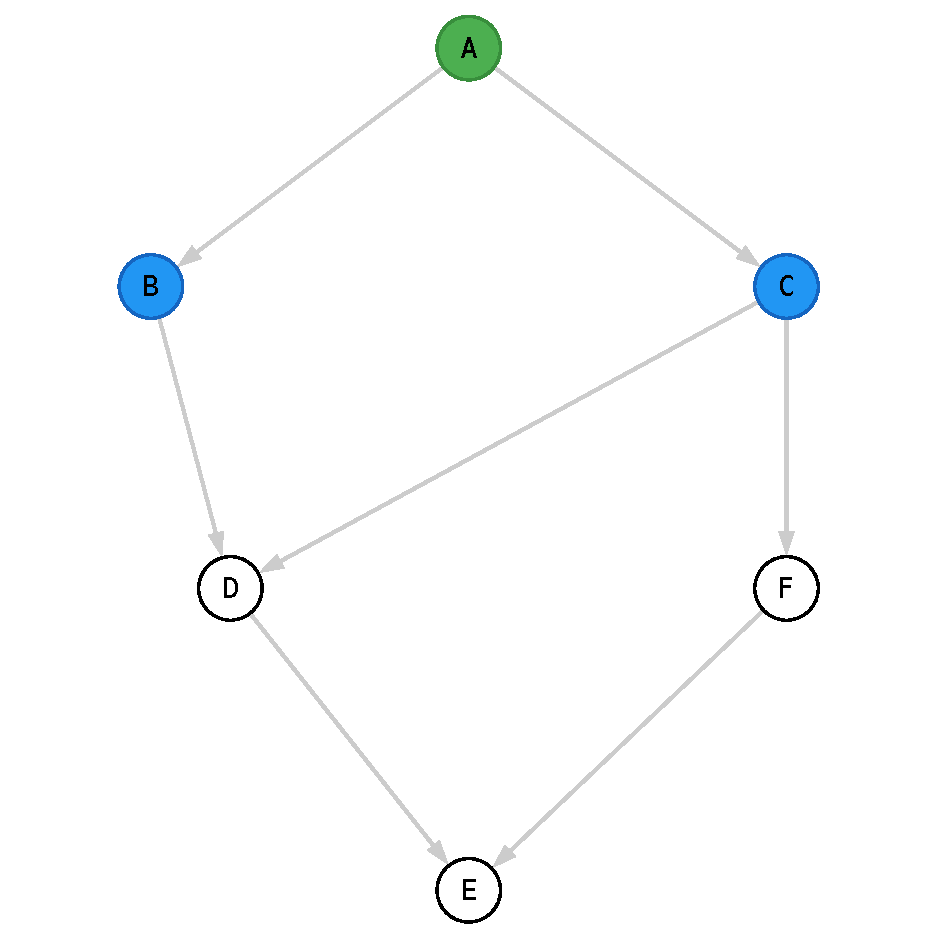
\includegraphics[width=0.30\textwidth]{python/lec02/topsort/topsort-1.pdf}\\[2pt]{\scriptsize Шаг 1. DFS из $A$: идём $A \to B$}} &
\shortstack{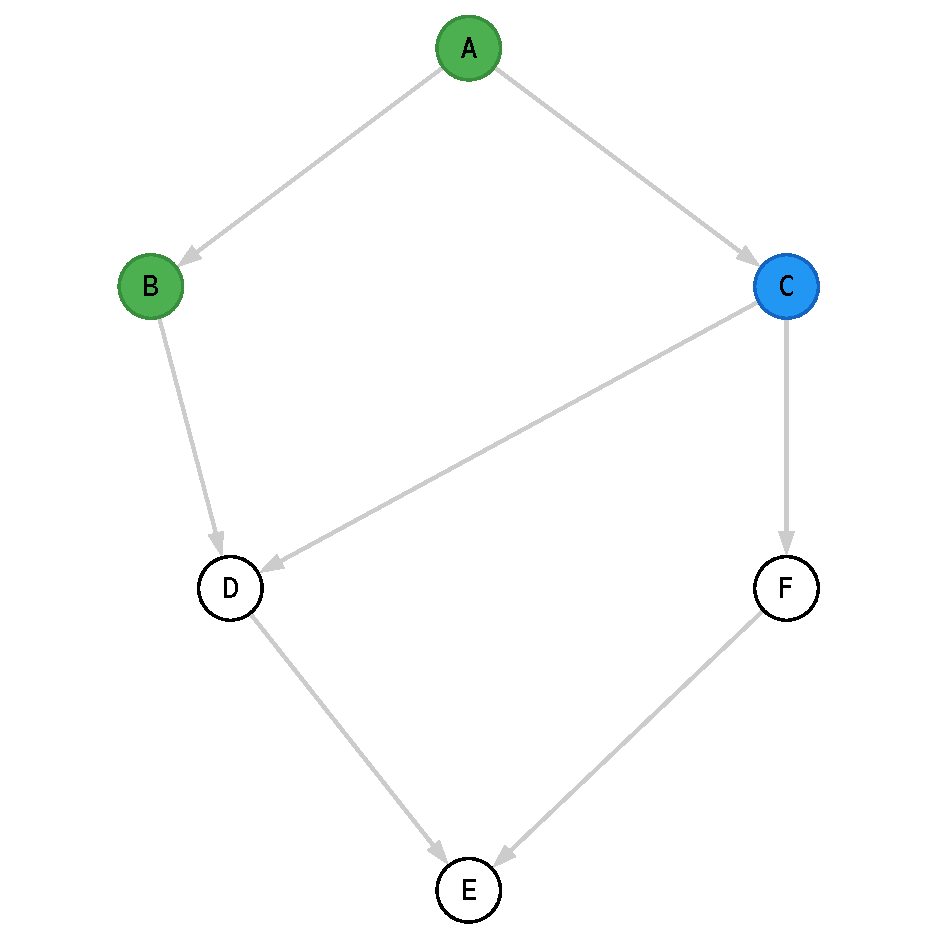
\includegraphics[width=0.30\textwidth]{python/lec02/topsort/topsort-2.pdf}\\[2pt]{\scriptsize Шаг 2. $B$ тупиковая $\to$ в стек}} \\
\end{tabular}\end{center}
\begin{center}\begin{tabular}{ccc}
\shortstack{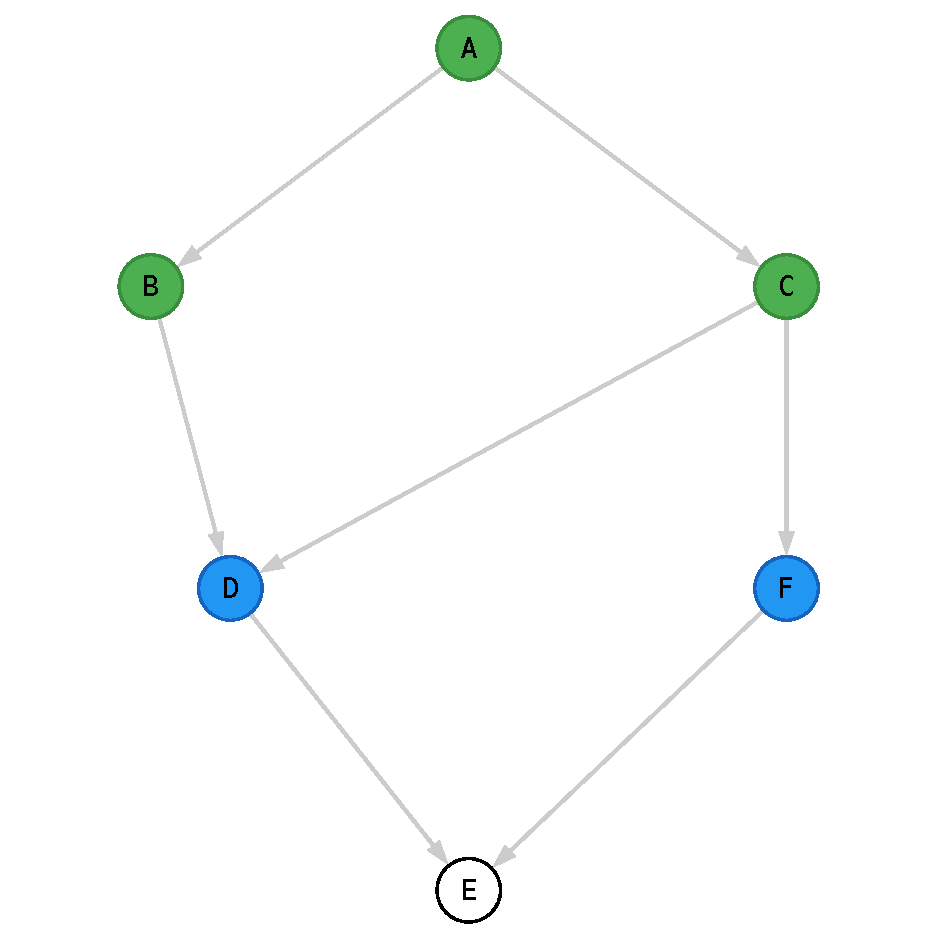
\includegraphics[width=0.30\textwidth]{python/lec02/topsort/topsort-3.pdf}\\[2pt]{\scriptsize Шаг 3. $A$ тупиковая $\to$ в стек}} &
\shortstack{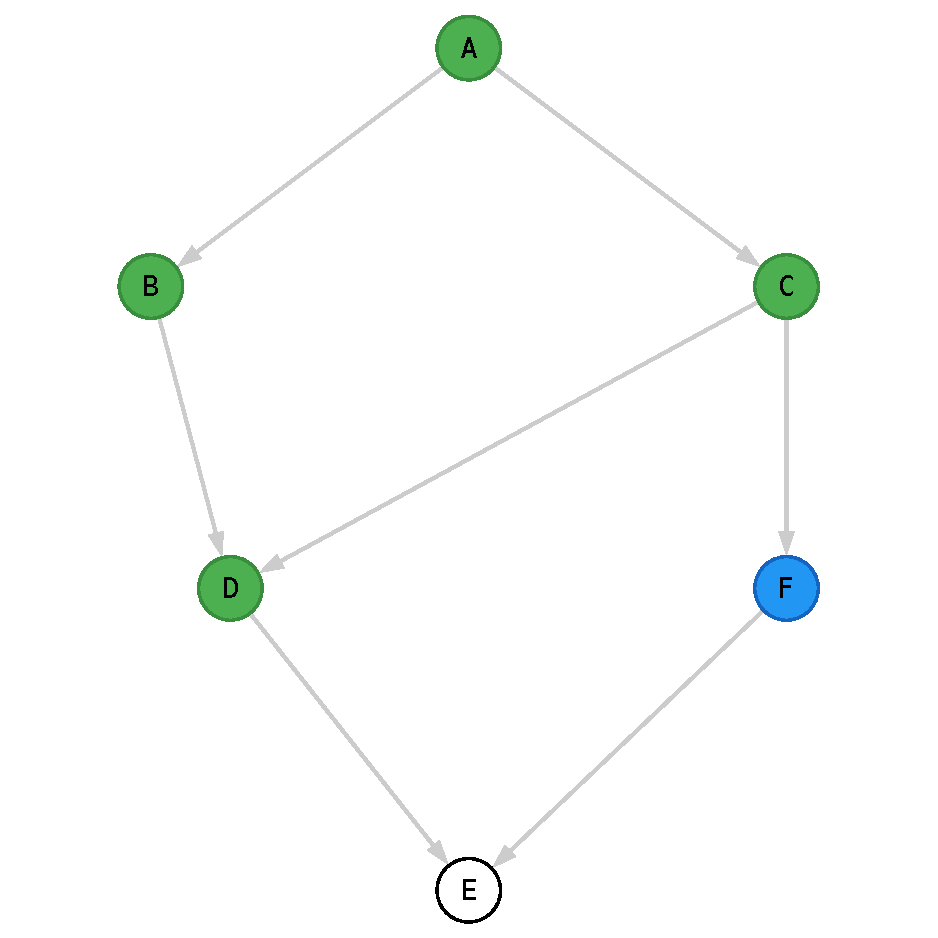
\includegraphics[width=0.30\textwidth]{python/lec02/topsort/topsort-4.pdf}\\[2pt]{\scriptsize Шаг 4. DFS из $C$: $C \to D$; $D \to$ в стек}} &
\shortstack{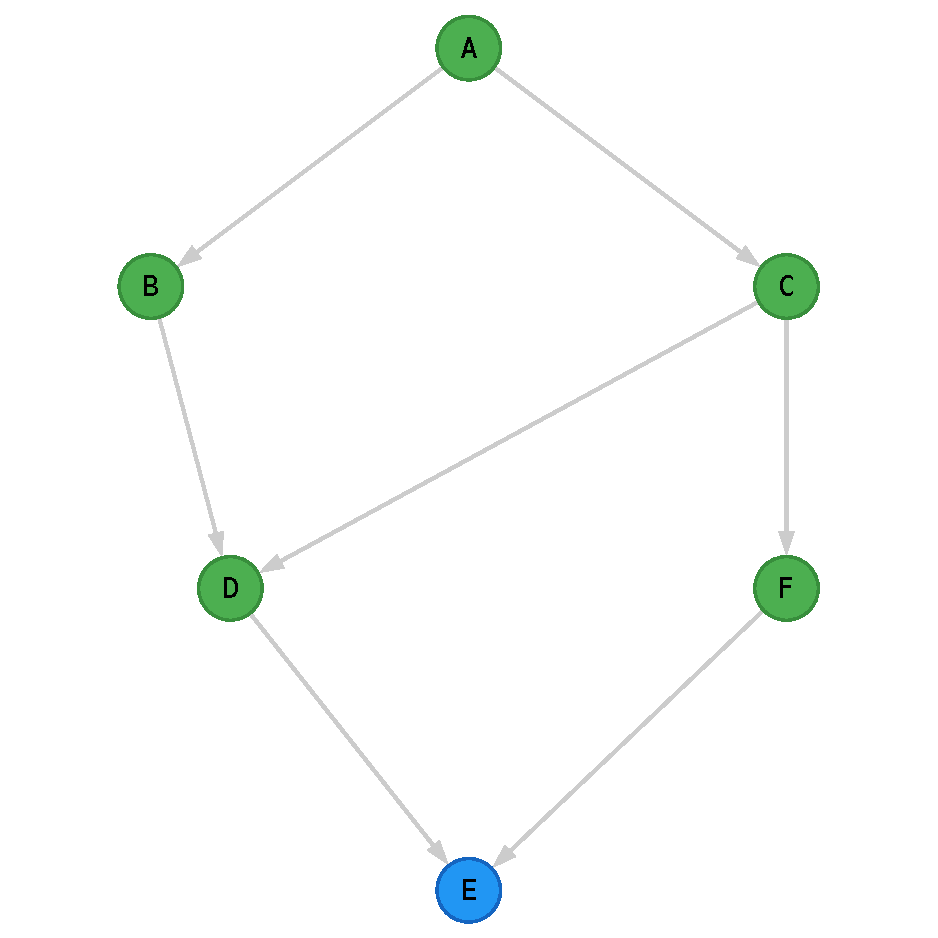
\includegraphics[width=0.30\textwidth]{python/lec02/topsort/topsort-5.pdf}\\[2pt]{\scriptsize Шаг 5. $C \to E$; $E \to$ в стек}} \\
\end{tabular}\end{center}
\begin{center}\begin{tabular}{ccc}
\shortstack{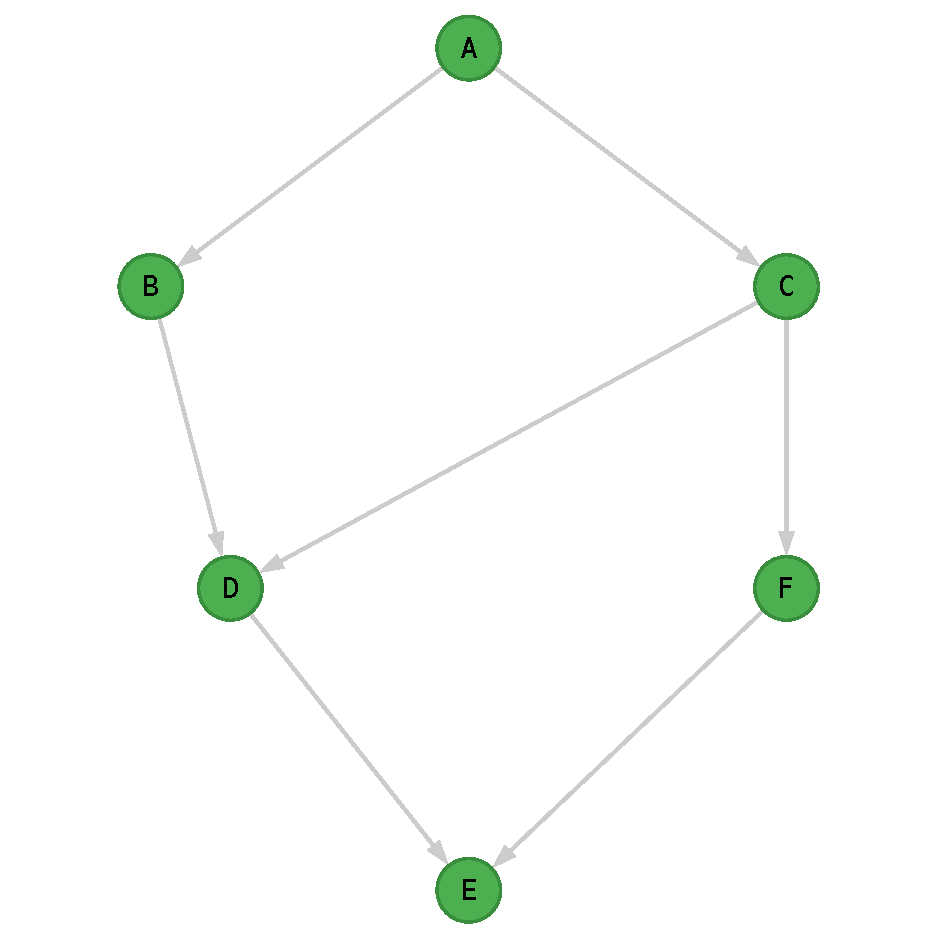
\includegraphics[width=0.30\textwidth]{python/lec02/topsort/topsort-6.pdf}\\[2pt]{\scriptsize Шаг 6. $C$ тупиковая; шаг I завершён}} &
\shortstack{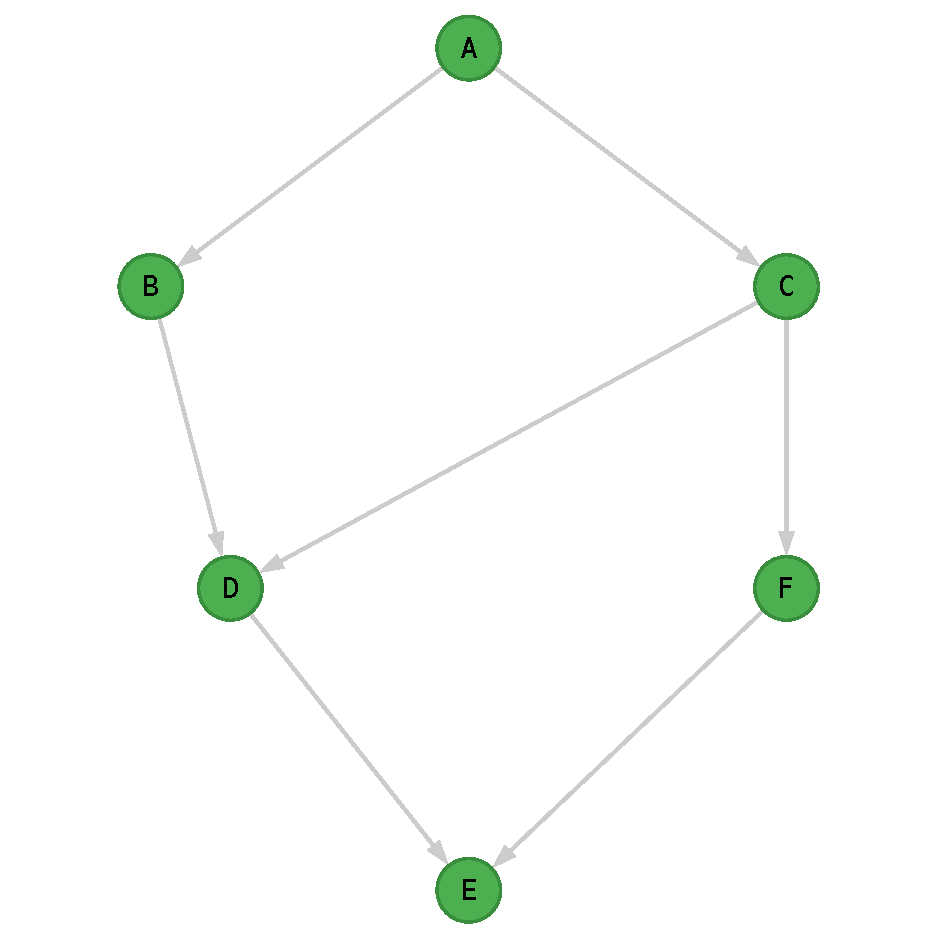
\includegraphics[width=0.30\textwidth]{python/lec02/topsort/topsort-7.pdf}\\[2pt]{\scriptsize Шаг 7. Нумерация по стеку + петли}} &
\shortstack{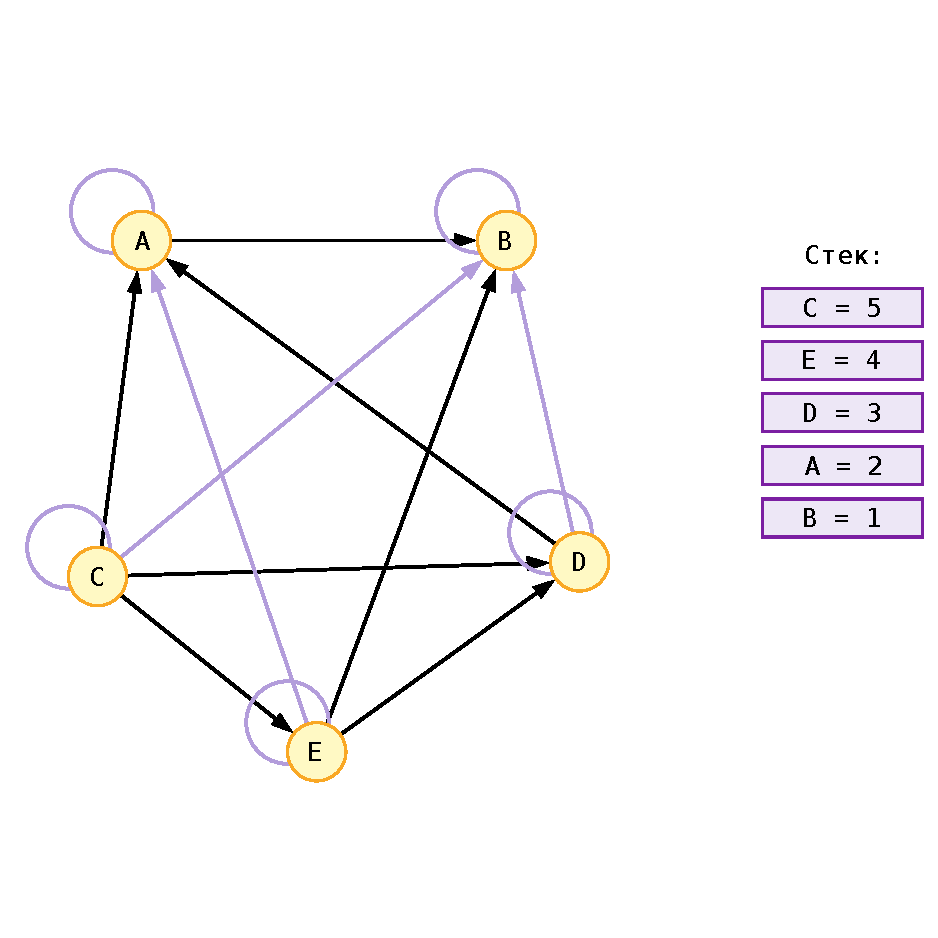
\includegraphics[width=0.30\textwidth]{python/lec02/topsort/topsort-8.pdf}\\[2pt]{\scriptsize Шаг 8. Недостающие рёбра}} \\
\end{tabular}\end{center}

\noindent\textit{Комментарии к шагам.}
На шаге~1 запускаем DFS из $A$: единственное исходящее ребро ведёт в $B$.
У $B$ исходящих рёбер нет --- она тупиковая, кладём её в стек (шаг~2);
возвращаемся в $A$ --- все её рёбра обработаны, $A$ тоже уходит в стек
(шаг~3). Запускаем DFS из следующей непосещённой вершины $C$: ребро
$C \to D$ приводит в $D$, откуда идёт только ребро $D \to A$ в уже
посещённую вершину, поэтому $D$ тупиковая (шаг~4). Далее $C \to E$:
оба ребра из $E$ ($E \to D$, $E \to B$) ведут в посещённые вершины ---
$E$ в стек (шаг~5). Наконец тупиковой становится и $C$ (шаг~6).

На шаге~7 нумеруем вершины по стеку снизу вверх:
$B = 1,\; A = 2,\; D = 3,\; E = 4,\; C = 5$ --- и дорисовываем
рефлексивные петли (светло-фиолетовые). На шаге~8 добавляем недостающие
рёбра из вершин с бóльшими номерами в вершины с меньшими (тоже
светло-фиолетовые: $D \to B$, $E \to A$, $C \to B$ и т.\,д.).

\medskip
Стек (низ $\to$ верх): $B, A, D, E, C$.

Нумерация вершин: $B = 1,\; A = 2,\; D = 3,\; E = 4,\; C = 5$.

Линейный порядок: $B \leq A \leq D \leq E \leq C$.

% Результат: topsort-result-0.graph
\grfig[0.45]{figures/topsort-result-0.pdf}{Результат Topsort --- линейный порядок $B \leq A \leq D \leq E \leq C$}
\end{algo}
